%===============================================================================
% ifacconf.tex 2025-07-31 jpuente  
% 2022-11-11 jpuente change length of abstract
% 2025-07-31 jldiez added section on the use of AI
% Template for IFAC meeting papers
% Copyright (c) 2025 International Federation of Automatic Control
%===============================================================================
\documentclass{ifacconf}

\usepackage{graphicx}      % include this line if your document contains figures
\usepackage{natbib}        % required for bibliography
\usepackage{xcolor}
\usepackage{subcaption}
\usepackage{siunitx}
\usepackage{amsmath,amssymb,amsfonts} 
%===============================================================================
\begin{document}
\begin{frontmatter}

\title{\textcolor{red}{Style for IFAC Conferences \& Symposia: Use Title Case for
  Paper Title}} 
% Title, preferably not more than 10 words.

\author[First,Second]{Alessandra Elisa Sindi Morando} 
\author[Second]{Jossué Cari\~no}
\author[Second]{Pedro Castillo} 
\author[First]{Roberto Sacile}
\author[First]{Enrico Zero}

\address[First]{
   \textit{University of Genoa}, Genoa, Italy \\
   alessandra.elisa.sindi.morando@edu.unige.it, roberto.sacile@unige.it, enrico.zero@dibris.unige.it
}
\address[Second]{
   \textit{Université de technologie de Compiègne}, CNRS, Heudiasyc, Compiègne, France \\
   alessandra-elisa-sindi.morando@utc.fr, \{jossue.escobar, pedro.castillo\}@hds.utc.fr
}

\begin{abstract}                % Abstract of 50--100 words
\textcolor{red}{\dots}
\end{abstract}

\begin{keyword}
   \textcolor{red}{\dots}
   %Five to ten keywords, preferably chosen from the IFAC keyword list.
\end{keyword}

\end{frontmatter}
%===============================================================================

\section{Introduction}
Multi-agent systems (MASs) are nowadays used in a variety of applications from as
they can perform complex tasks, which would otherwise impossible for a single robot.
This is even more the case when considering heterogeneous fleet where the strenghts
of one type of robot can compensate for the limitations of another.
For example, to monitor a large area, multiple ground agents can move from one point 
to another being supervised from above by a drone with a wide field of view.
To deepen the subject and understand both the potential tasks and challenges of MASs,
the reader can refer to the work of~\cite{Maldonado2024}.

One of the fundamental cooperative tasks when working with multi-agents is formation
control.
This topic has been studied for years.
For example, already~\cite{LEE200985} already proposed
a decentralized control algorithm for a team of two-wheeled robots 
to achieve achieve a geometric pattern.
However, formation control remains an hot challenging topic to this day.
\cite{TRAN2021100117} experimentally validated a robust distributed control 
based on negative imaginary systems consensus theory, using both ground robots and
an air-ground fleet.
In the work of~\cite{GULER2023105492}, each agent computes its control action 
in a leader-follower manner using local extended Kalman filter's estimates to 
achieve a desired shape together with other wheeled robots and a drone.
An optimal distributed formation control algorithm for double-integrator multi-agents
has been presented and validated through simulations by~\cite{Huang2023}.
\cite{Aditya2023} defined the formation problem for a group of double-integrator agents 
as a discrete-time game whose solution is given by a state-dependent Riccati equation.
A robust distributed consensus controller is presented by~\cite{Restrepo2023}
to address the rendezvous problem and applied in simulation to a swarm of drones.
In the recent years, reinforcement learning has used in many areas including 
formation control. 
\cite{WANG20208150} addressed multi-particle formation control by combining 
graph attention networks and multiple long short-term memories to achieve the 
desired shape and avoid collisions respectively.
A position and an orientation robust controllers based on reinforcement learning 
are proposed and validated through simulations by~\cite{Zhong2025} for the formation 
of a term of quadrotors.

In this context is placed this work which proposes a novel formation control scheme
for a team consisting of a quadcopter and two unicycles, as show in Fig.~\ref{fig:summary_image}.
\begin{figure}
    \centering
    % trim = left bottom right top (in points or any unit)
    % clip = true ensures the parts outside the box are hidden
    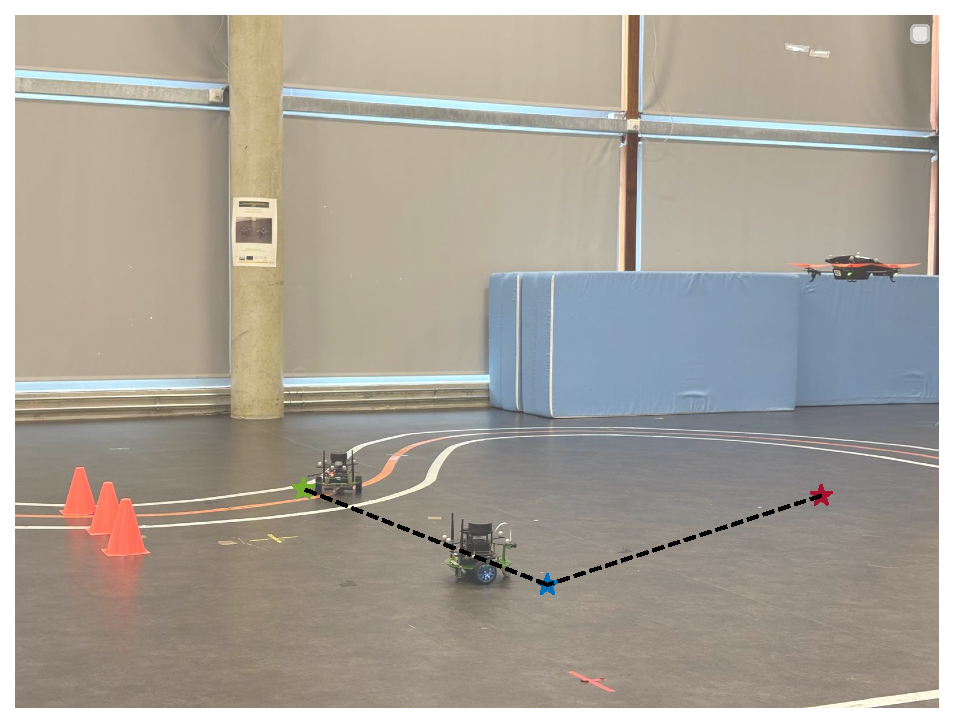
\includegraphics[width=0.9\columnwidth, trim=10 50 15 110, clip]{images/output.pdf}
    \caption{This paper proposes a formation control for a heterogeneous fleet to attain a desired shape despite obstacles.}
    \label{fig:summary_image}
    \vspace{-0.1cm}
\end{figure}
When addressing the multi-agent formation, there are two main challenges to solve: 
achieving the desired shape and avoiding collisions.
On one hand, for the first challenge, a distributed controller combining Feedback 
Linearization (FL) and an optimal linear controller based on Linear Matrix 
Inequalities (LMIs) is presented.
LMIs are a powerful mathematical tool used in many applications among which also 
formation control.
In the work of~\cite{Trejo2023}, an LMI is solved to design the controller 
and observer gains, guaranteeing stable formation flight for a group of quadcopters.
~\cite{Deshpande2011} propose a formation control with artificial 
fixed delays for multiple double-integrators and 
verify the asymptotic stability of the scheme by checking 
the solvability of an LMI.
~\cite{Semsar2009} present an LMI formulation of the LQR problem 
to guarantee stable state consensus with an optimal control effort 
in a multi-agent system.
On the other end, to avoid collision avoidance, the chosen solution is 
Artificial Potential Field (APF).
In analogy with a particle moving in an electrostatic or gravitational
field, virtual repulsive force fields are simulated to ward off the robot
from an obstacle.
This approach has been widely used in formation control of ground vehicles,
see for example the work of~\cite{Yongshen2018}.
However, in more recent works, e.g.~\cite{HAN2024106105} and~\cite{Piet2025Control},
APFs are employed to navigate around obstacles and prevent collisions 
while attaining the desired shape.
% \textcolor{red}{
% \begin{itemize}
%    %  \item survey on multi-agent systems~\cite{Maldonado2024}
%    %  \item other works on air-ground cooperation:
%    %  \item works on obstacle avoidance and formation:
%    %  ~\cite{WANG20208150},
%    %  ~\cite{TRAN2021100117} (air-ground),
%    %  ~\cite{GULER2023105492}(air-ground, adaptive distributed leader-follower controller for formation),
%    %  ~\cite{Huang2023}(optimal algoritm, as me, and control barrier function),
%    %  ~\cite{Restrepo2023}(UAVs formation, collision vaoidance guaranteed with constraints),
%    %  ~\cite{Aditya2023}(double integrator Riccati equation for formation and collision avoidance)
%    %  ~\cite{LEE200985},
%    % \item LMI:
%    % ~\cite{Deshpande2011}(LMI  double integrator formation),
%    % ~\cite{Trejo2023}(use LMI to find controller gains for UAVs formation), 
%    % ~\cite{Semsar2009}(LMI to optimal consensus multi-agent)
%    %  \item other works with APF:
%    %  ~\cite{Yongshen2018}(applied to UGVs),
%    %  ~\cite{Piet2025Control, HAN2024106105} (both applied to drones)
%     \item previous work:~\cite{Morando2025SOSE}
% \end{itemize}
% }

This paper represents the continuation of the previous work by~\cite{Morando2025SOSE},
where a control architecture combining Feedback Linerarization (FL), 
a robust LMI-based controller and APFs was proposed 
and validated through simulations for 
the formation of three unicycles.
The successive developments sought to manage the challenge
of a heterogeneous team (replacing a ground vehicle with a quadcopter)
by adapting the methodology and then experimentally validating 
the new solution.
The contributions of this work are: a) a controller involving FL, a LMI-based controller and APFs 
is presented for the stable formation of an air-ground fleet;
b) the proposed controller has been validated through MATLAB Simulink
simulations and a comprensive set of experiments, including both static
and dynamic obstacle scenarios.
The remainder paper is structured as follows. 
In Section~\ref{sec:heterogeneous_fleet_modeling}, 
the mathematical model used to describe the team is stated.
The proposed formation controller is detailed in Section~\ref{sec:formation_controller}.
The simulations and experiments results are reported and analyzed
in Section~\ref{sec:simulation_results} and 
in Section~\ref{sec:experimental_validation} respectively.
Finally, conclusions are drawn in Section~\ref{sec:conclusion}.

\section{Heterogeneous Fleet Modeling}
\label{sec:heterogeneous_fleet_modeling}
In this section, the dynamics of the agents composing the team
(i.e., of the two unicycles and the quadrotor, as shown in Fig.~\ref{fig:airground-fleet}.)
are described and adapted to then apply the LMI approach.
\begin{figure}
    \centering
   %  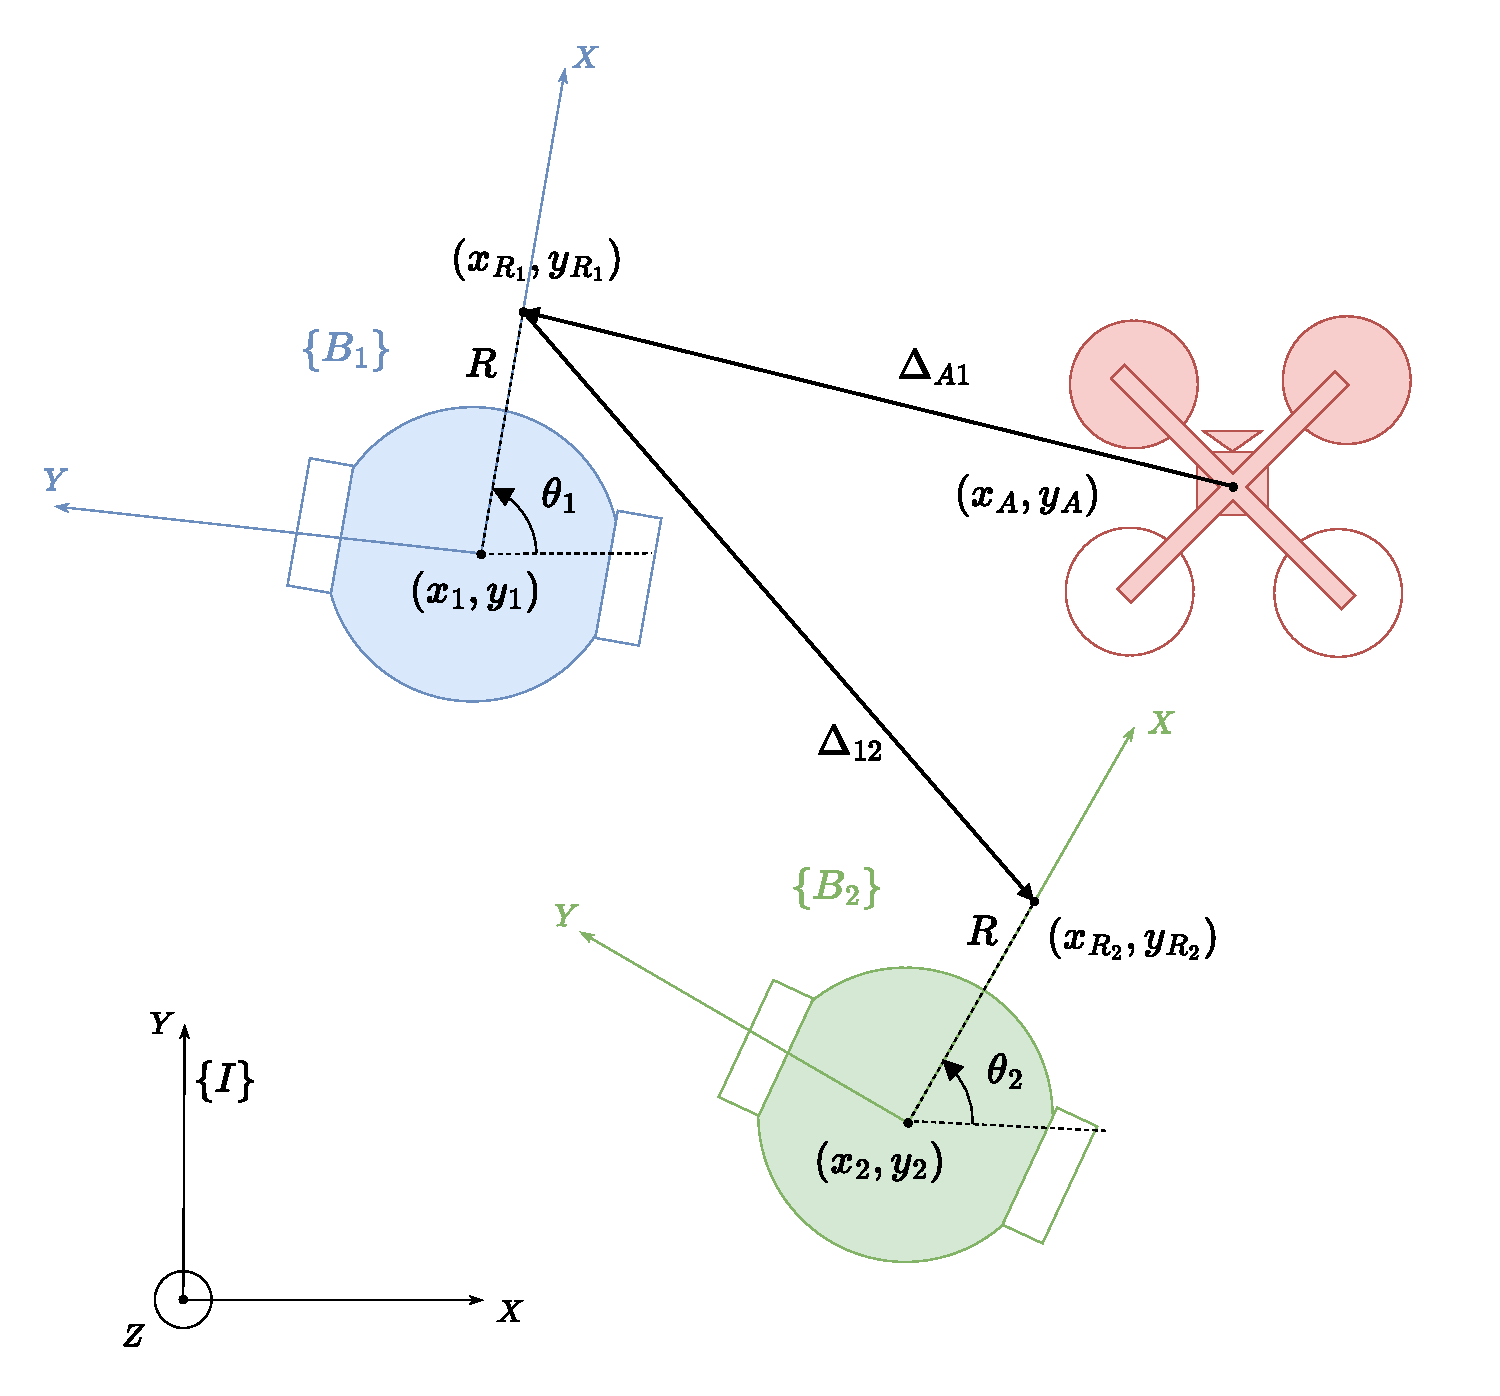
\includegraphics[height=6cm]{images/heterogenous_fleet.pdf}
    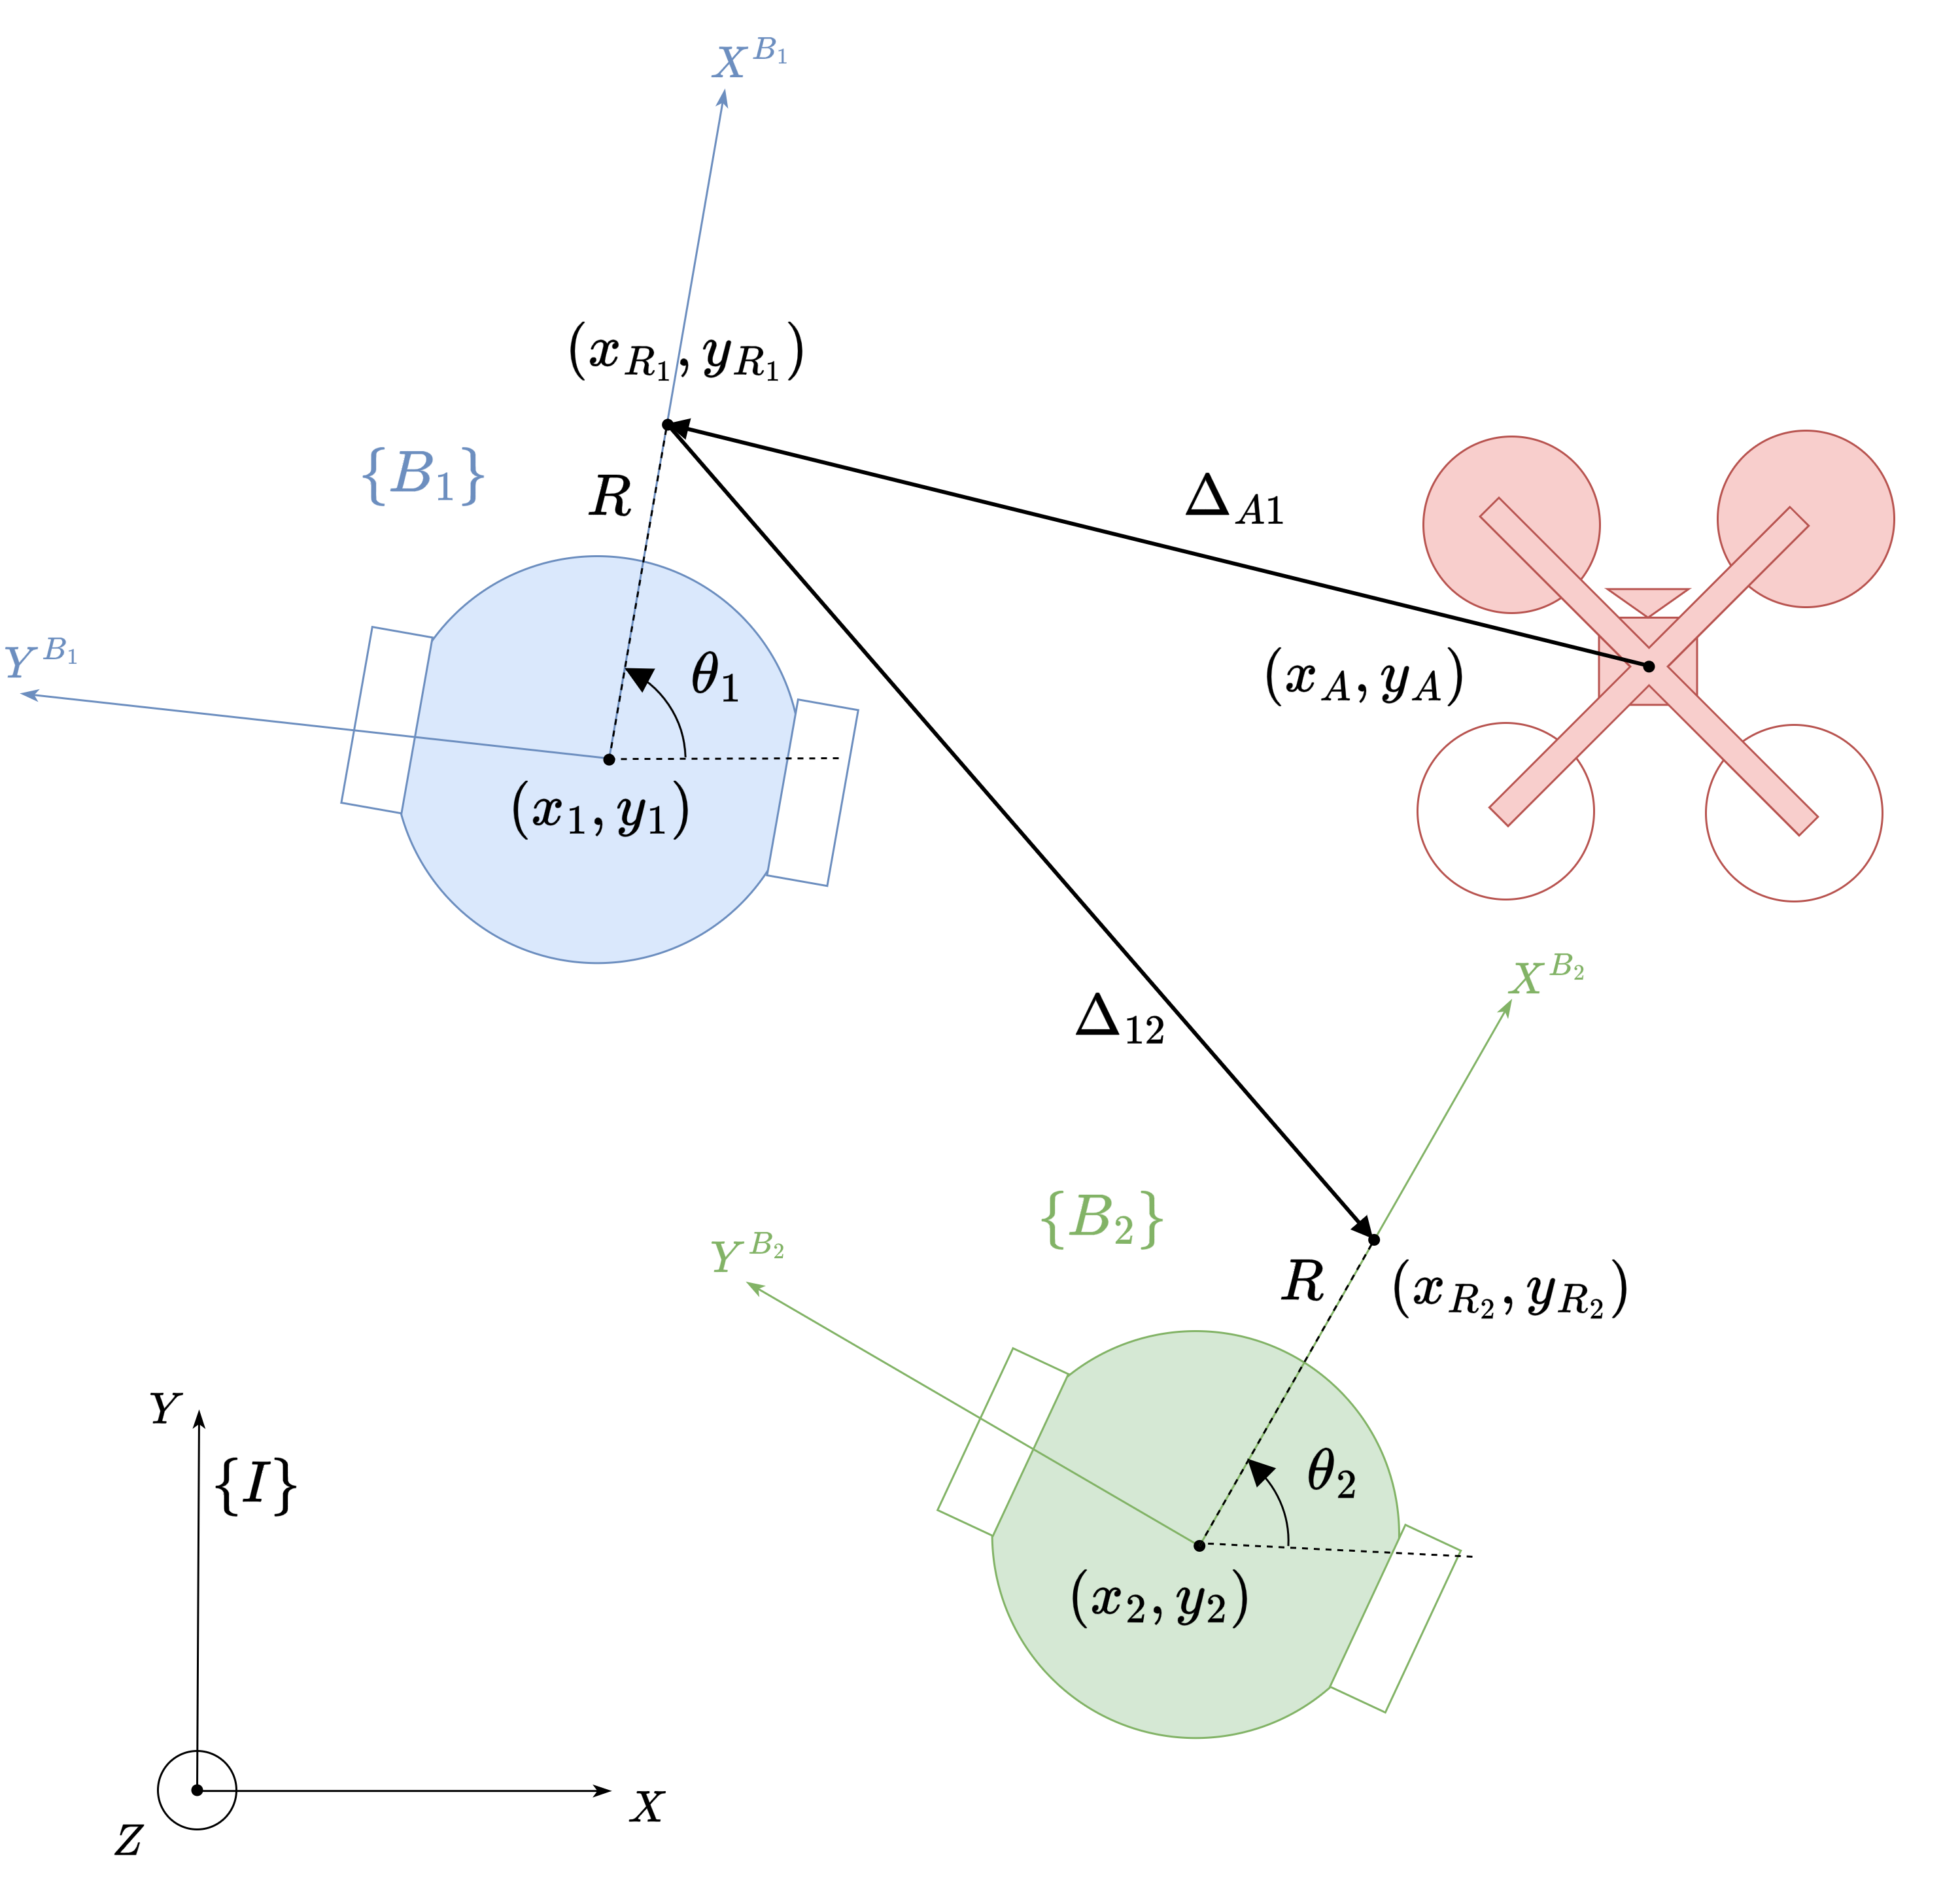
\includegraphics[height=6.1cm]{images/heterogenous_fleet_PNG300_2.png}
    \caption{Air-ground heterogeneous fleet.}
    \label{fig:airground-fleet}
\end{figure}
The well-known kinematic model of a two-wheeled robot $R_i$ is
\begin{equation}
    \begin{cases}
        \dot{x}_i &= v_i \, \cos\theta_i \\
        \dot{y}_i &= v_i \, \sin\theta_i \\
        \dot{\theta}_i &= \omega_i
    \end{cases}
    \label{eq:unicycle_i_t-model}
\end{equation}
where $(x_i, y_i, \theta_i)$ is the pose of the agent 
and $(v_i, \omega_i)$ are the linear and
angular velocities respectively.
The equations~\eqref{eq:unicycle_i_t-model} describing the motion of the center of rotation are non-linear.
But still, if a point located at distance $R > 0$ from 
$(x_i, y_i)$ denote as $({x}_{R_i}, {y}_{R_i})$, is 
considered and new virtual inputs are defined $(u_{i,x},u_{i,y})$, 
the dynamics become linear:
\begin{equation}
    \begin{cases}
        \dot{x}_{R_i} = u_{i,x} \\
        \dot{y}_{R_i} = u_{i,y} \\
    \end{cases}
\end{equation}
Moving on to the drone, as in the formation problem deals with the $(X,Y)$-dynamics, some simplifying hypothesis have been made.
First, let us assume that there is an inner attitude controller.
Hence, the focus is only on the translational dynamics which are:
\begin{equation}
    \begin{cases}
        m\ddot{x}^F_A = - T \sin \theta \\
        m\ddot{y}^F_A = T \cos \theta \sin \phi \\
        m\ddot{z}^F_A = T \cos \theta \cos \phi  - m\, g\\
    \end{cases}
\end{equation}
Let analyze the equations with the help of Fig.~\ref{fig:drone_roll_pitch_frames}.
The state $({x}^F_A,{y}^F_A,{z}^F_A)$ represents the position of the drone w.r.t. the inertial frame $\{F\}$.
The frame $\{F\}$ has been used instead of $\{I\}$ to be aligned with the framework employed 
to implement the controller for the drone, see Section~\ref{sec:experimental_validation}.
The angles $\phi$ and $\theta$ are the roll and pitch Euler angles 
of the body frame $\{B\}$ (fixed to the drone) relative to the inertial
frame $\{F\}$.
Ignoring the small body forces, the only forces acting on the drone are 
the trust produced by the motors $T$ along the $k^B$ direction and 
the gravity $mg$ along the $-k^F$ direction.
\begin{figure}
    \centering
    \begin{subfigure}{0.31\columnwidth}
        % trim = left bottom right top (in points or any unit)
        \hspace{0.5cm}
        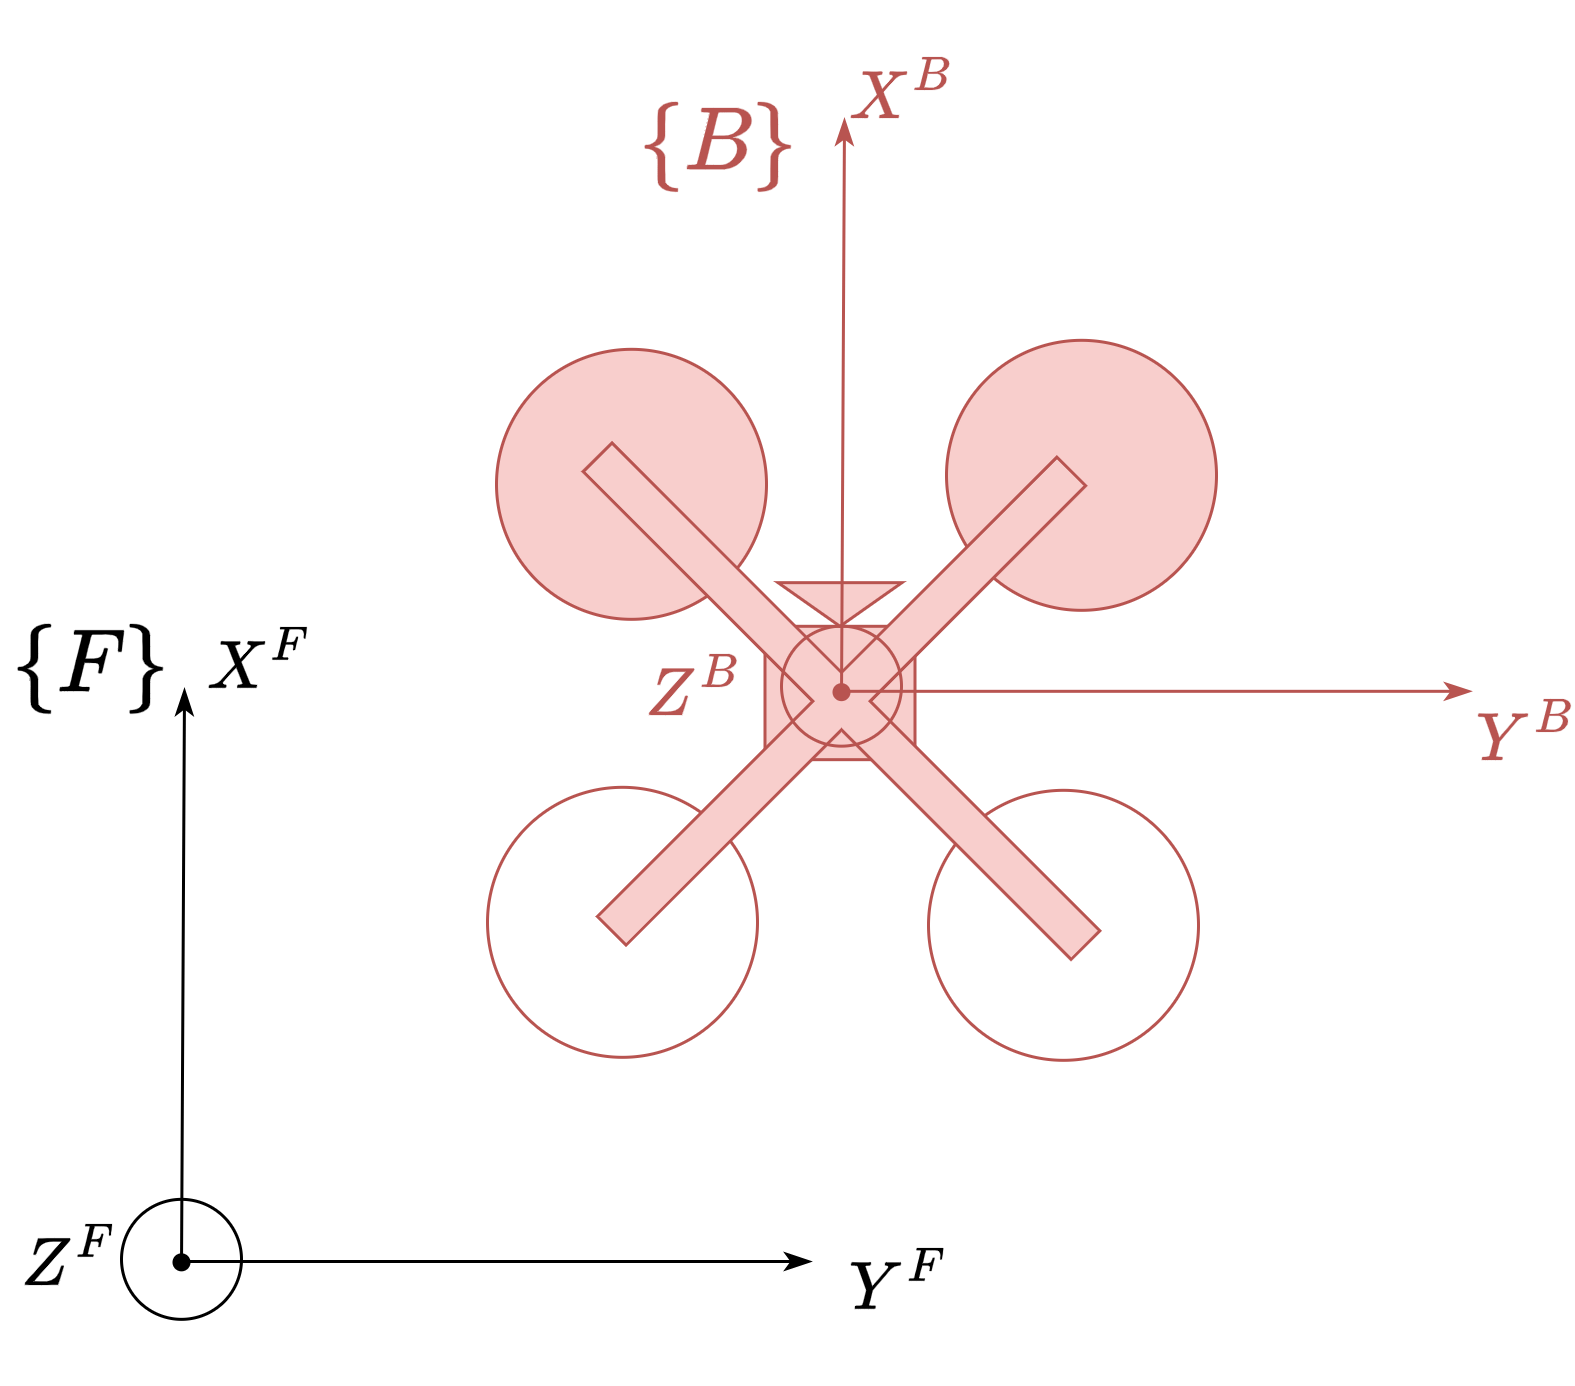
\includegraphics[trim={0.8cm 2cm 0cm 2cm}, clip, width=3cm]{images/drone_fromAbove2.png}
        % \caption{Drone's body frame $B$ and FL-AIR frame $F$.}
    \end{subfigure}
    \hfill
    \begin{subfigure}{0.31\columnwidth}
        \hspace{0.5cm}
        % 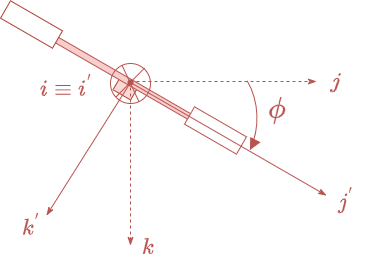
\includegraphics[trim={0.8cm 0.4cm 0cm 0.5cm}, clip, width=3cm]{images/drone_roll.png}
        % \vspace{-1.3cm}
        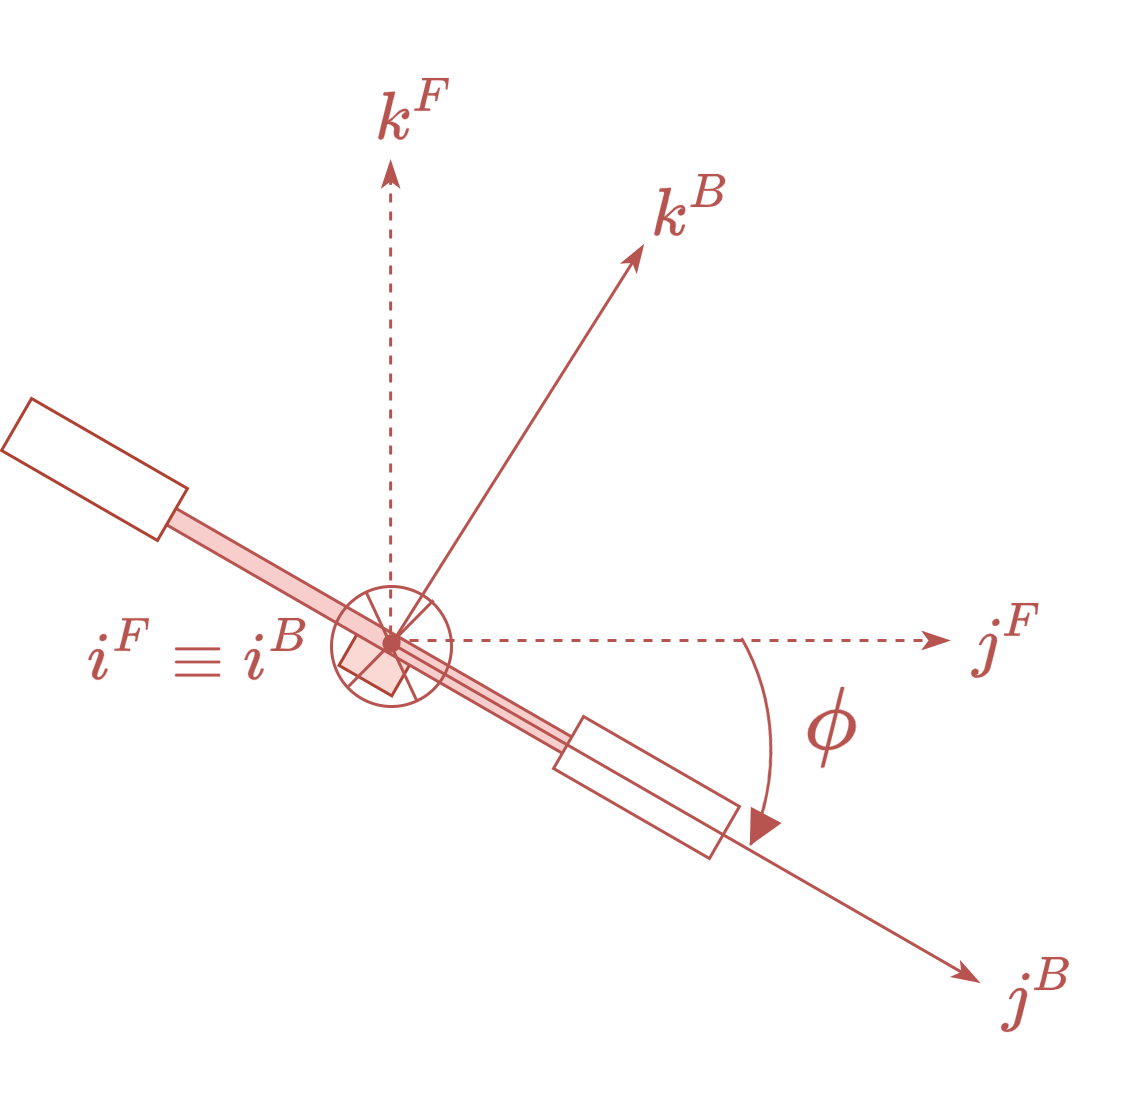
\includegraphics[trim={0cm 0cm 0.5cm 0cm}, clip, width=3cm]{images/drone_roll3.png}
        % \vspace{0.7cm}
        % \caption{Roll $\phi$ w.r.t  the frame $B$.\\}
    \end{subfigure}
    \hfill
    \begin{subfigure}{0.31\columnwidth}
        \hspace{0.3cm}
        \vspace{0.5cm}
        % 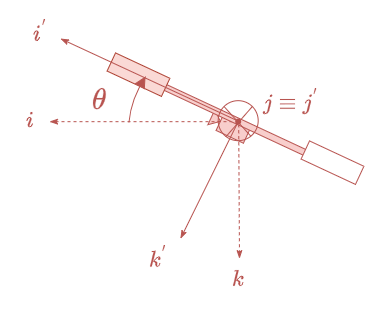
\includegraphics[trim={0cm 0cm 0.5cm 0cm}, clip, width=3cm]{images/drone_pitch.png}
        % \vspace{0.9cm}
        % \vspace{-0.01cm}
        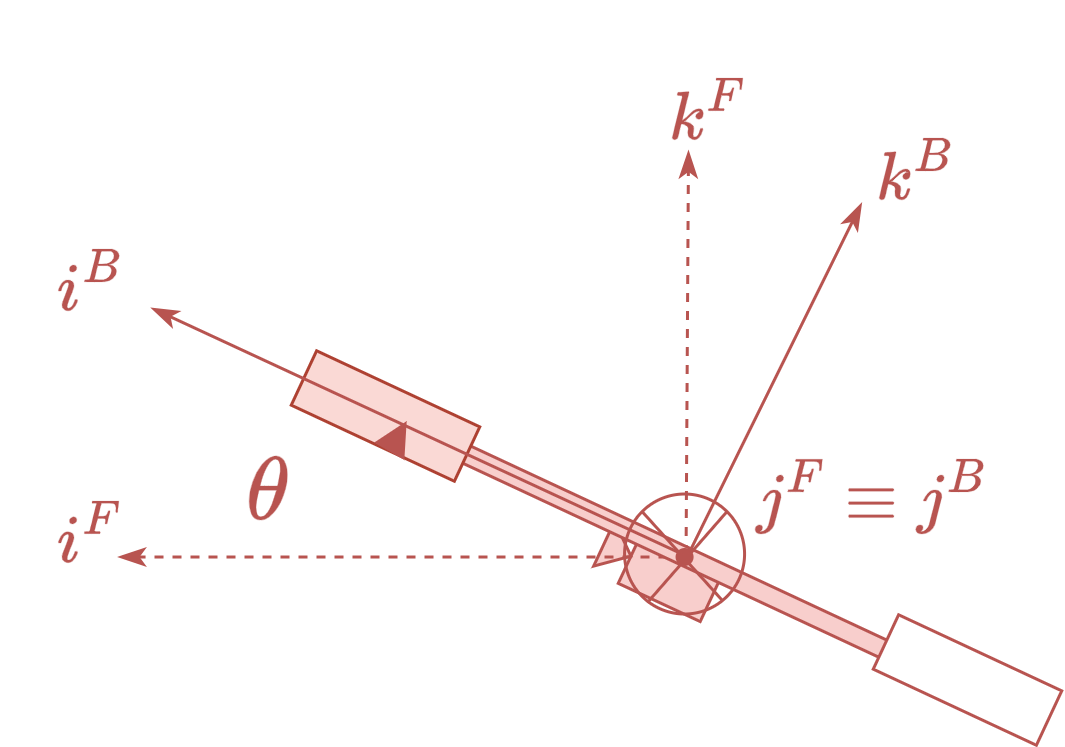
\includegraphics[trim={0.8cm 0.1cm 0cm 0.5cm}, clip, width=3cm]{images/drone_pitch2.png}
        % \vspace{0.1cm}
        % \vspace{0.9cm}
        % \caption{Pitch $\theta$ w.r.t  the frame $B$.\\}
    \end{subfigure}
    \caption{Quadcopter's roll $\phi$ and pitch $\theta$ angles.} 
    \label{fig:drone_roll_pitch_frames}
\end{figure}
Let suppose that the $Z$-controller 
\begin{equation}
    T = (r_1 + mg) / (\cos \phi \cos \theta)
\end{equation}
is such that the drone's mass is compensated in a short time
by $r_1$, i.e. $r_1 \to 0$.
This implies that the $(x,y)$-dynamics will not include the mass of the drone,
as the $Z$-controller already compensated it.
Finally, let us make the hypothesis that the roll and pitch angles 
are small, i.e. $\phi,\theta \approx 0$.
Then, the translational dynamics simplify to 
\begin{equation}
    \begin{cases}
        \ddot{x}^F_A = -g\theta \\
        \ddot{y}^F_A = g\phi
    \end{cases}
    \label{eq:drone_t-model}
\end{equation}
At this point, all the agents can be described by the linear models
\eqref{eq:unicycle_i_t-model} and~\eqref{eq:drone_t-model}.
To define the formation problem, let us introduce the quantities
\begin{subequations}
    \begin{equation}
        \Delta_{A1} = \begin{bmatrix}
            \Delta_{A1,x} & \Delta_{A1, y}
        \end{bmatrix}^T 
    \end{equation}
    \begin{equation}
        \Delta_{A1,x} = x_{R_1} - x_A = x_{R_1} - y^F_A \  
    \end{equation}
    \begin{equation}
        \Delta_{iA,y} = y_{R_1} - y_A = y_{R_1} - x^F_A
    \end{equation}
\end{subequations}
with $(x_A, y_A)$ the position of the drone w.r.t the inertial frame $\{I\}$,
\begin{subequations}
    \begin{equation}
        \Delta_{A1} = \begin{bmatrix}
        \Delta_{A1,x} & \Delta_{A1, y}
    \end{bmatrix}^T 
    \end{equation}
    \begin{equation}
        \Delta_{A1,x} = x_{R_1} - x_A = x_{R_1} - y^F_A
    \end{equation}
    \begin{equation}
        \Delta_{iA,y} = y_{R_1} - y_A = y_{R_1} - x^F_A
    \end{equation}
\end{subequations}
the desired inter-distances $ \Delta^d_{A1}$ and $\Delta^d_{12}$,
 and the desired position of the drone $(x^d_A, y^d_A)$ w.r.t the inertial 
 frame $\{I\}$ (constant over time).
The overall dynamics of the formation's errors are as follows
\begin{equation}
\begin{cases}
    \ddot{e}_{A,x} = - g \theta \\
    \ddot{e}_{A,y} = g \phi \\
    \dot{e}_{\Delta_{A1,x}} = u_{1,x}  - \dot{e}_{A,y} \\
    \dot{e}_{\Delta_{A1,y}} = u_{1,y}  - \dot{e}_{A,x} \\
    \dot{e}_{\Delta_{12, x}} = u_{2,x}  - u_{1,x} \\
    \dot{e}_{\Delta_{12, y}} = u_{2,y}  - u_{1,y}
\end{cases}
\label{eq:airground-continous_time-sys}
\end{equation}
with 
\begin{equation}
e_{A,x} = x^F_A - y^d_A, \ e_{A,y} = y^F_A - x^d_A
\end{equation}
\begin{equation}
e_{\Delta_{A1,x}} = \Delta_{A1,x} - \Delta^d_{A1,x}, \ 
e_{\Delta_{A1,y}} = \Delta_{A1,y} - \Delta^d_{A1,y}
\end{equation}
\begin{equation}
e_{\Delta_{12,x}} = \Delta_{12,x} - \Delta^d_{12,x}, \ 
e_{\Delta_{12,y}} = \Delta_{12,y} - \Delta^d_{12,y}
\end{equation}
Let us define the state and control vectors as follows
\begin{subequations}
    \begin{equation}
        \footnotesize
        \boldsymbol{e}^T = \begin{bmatrix}
            e_{A,x} & \dot{e}_{A,x} & e_{A,y} & \dot{e}_{A,y} 
            & e_{\Delta_{A1,x}} & e_{\Delta_{A1,y}}
            & e_{\Delta_{12,x}} & e_{\Delta_{12,y}}
        \end{bmatrix}
    \end{equation}
    \begin{equation}
        \boldsymbol{u}_A = \begin{bmatrix}
            \phi  \\ \theta 
        \end{bmatrix}, \
        \boldsymbol{u}_1 = \begin{bmatrix}
            u_{1,x} \\ u_{1,y}
        \end{bmatrix}, \ 
        \boldsymbol{u}_2 = \begin{bmatrix}
            u_{2,x} \\ u_{2,y}
        \end{bmatrix}, 
        \boldsymbol{u} = \begin{bmatrix}
            \boldsymbol{u}_A \\ \boldsymbol{u}_1 \\  \boldsymbol{u}_2
        \end{bmatrix}
        \label{eq:airground-continous_time-controls}
    \end{equation}
\end{subequations}
Hence, the heterogeneous fleet's dynamics can be written in a matrix form:
\begin{equation}
    \dot{\boldsymbol{e}} = A \boldsymbol{e} + B \boldsymbol{u}
\end{equation}
By discretizing with sampling time $\Delta T$ using the Euler method:
\begin{equation}
    \boldsymbol{e}(k+1) = A_d \boldsymbol{e}(k) + B_d \boldsymbol{u}(k) 
    \label{eq:airground-fleet-z}
\end{equation}
with $A_d = I + \Delta T A $ and $B_d = \Delta T B$.
To model real-world disturbances, it is assumed 
that an addictive zero-mean disturbance $\boldsymbol{d}(k)$
is acting on the input channel, i.e.
\begin{equation}
    \boldsymbol{e}(k+1) = A_d \boldsymbol{e}(k) + B_d \boldsymbol{u}(k) + B_d \boldsymbol{d}(k)
    \label{eq:airground-fleet-z}
\end{equation}
Let us make the following hypothesis: 
a) the drone knows its position;
b) the robot $R_1$ knows its position w.r.t the quadcopter;
c) the robot $R_2$ knows its position w.r.t the other agent $R_1$;
d) all unicycles are aware of their distance from any obstacles on the ground;
e) a hierarchy is defined between the ground robots: $R_1$ has the priority over $R_2$.
\section{Formation Controller}
\label{sec:formation_controller}

This section aims to detail the proposed formation controller.
The two crucial issues, formation maintenance and collision avoidance, 
are addressed respectively in the next two subsections.


\subsection{Formation Maintenance: an LMI Approach}
The first goal is to ensure the robots achieve the desired shape 
while using only local measurements 
and counteracting the worst-case disturbance.
Based on the previous hypotheses, the measurements of 
each agent are as follows:
\begin{subequations}
    \begin{equation}
    \boldsymbol{z}_A = \begin{bmatrix}
        e_{A,x}  \\ e_{A,y} \\ \dot{e}_{A,x} \\ \dot{e}_{A,x}
    \end{bmatrix}= C_A \, \boldsymbol{e}
\end{equation}
\begin{equation}
    \boldsymbol{z}_1 = \begin{bmatrix}
        e_{\Delta_{A1,x}} \\ e_{\Delta_{A1,y}}
    \end{bmatrix} = C_1 \, \boldsymbol{e}, \  
     \boldsymbol{z}_2 = \begin{bmatrix}
        e_{\Delta_{12,x}} \\ e_{\Delta_{12,y}}
    \end{bmatrix} = C_2 \, \boldsymbol{e}
\end{equation}
\label{eq:airground-continous_time-measurement}
\end{subequations}


\subsection{Obstacle Avoidance: APFs}


\section{Simulations Results}
\label{sec:simulation_results}
\begin{figure}
    \centering
   %  \hspace{1cm}
    \begin{subfigure}{0.3\columnwidth}
        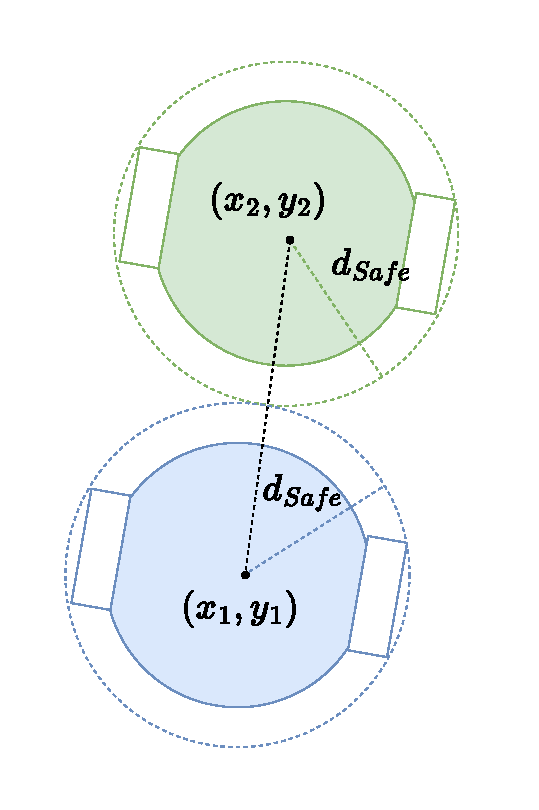
\includegraphics[height=3cm]{images/dSafe.pdf}
    \end{subfigure}
    \hspace{-0.6cm}
    \begin{subfigure}{0.3\columnwidth}
        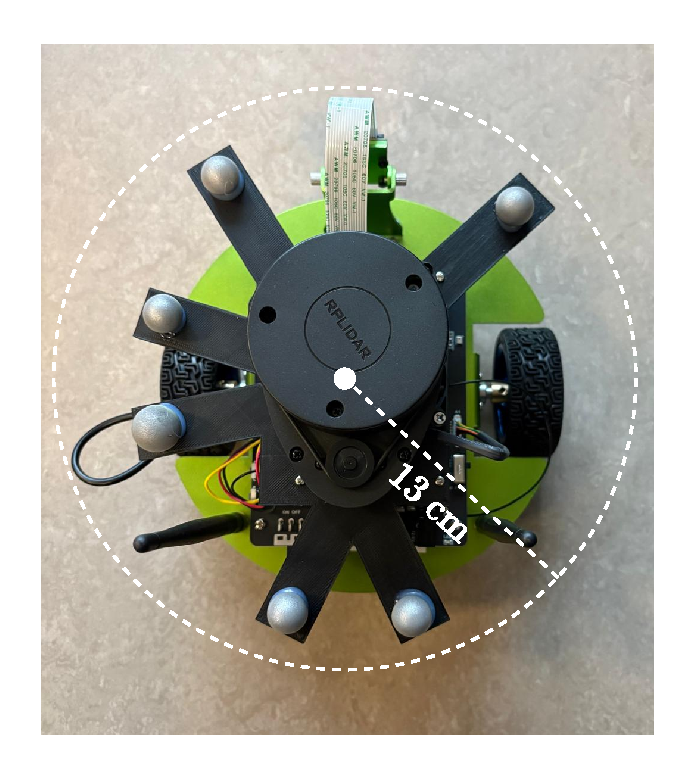
\includegraphics[height=3cm]{images/robot_dSafe.pdf}
    \end{subfigure}
    \caption{\textcolor{red}{TODO}}
    \label{fig:safety_distance}
\end{figure}
\begin{figure}
    \centering
    \begin{subfigure}[b]{0.32\columnwidth}
        \centering
        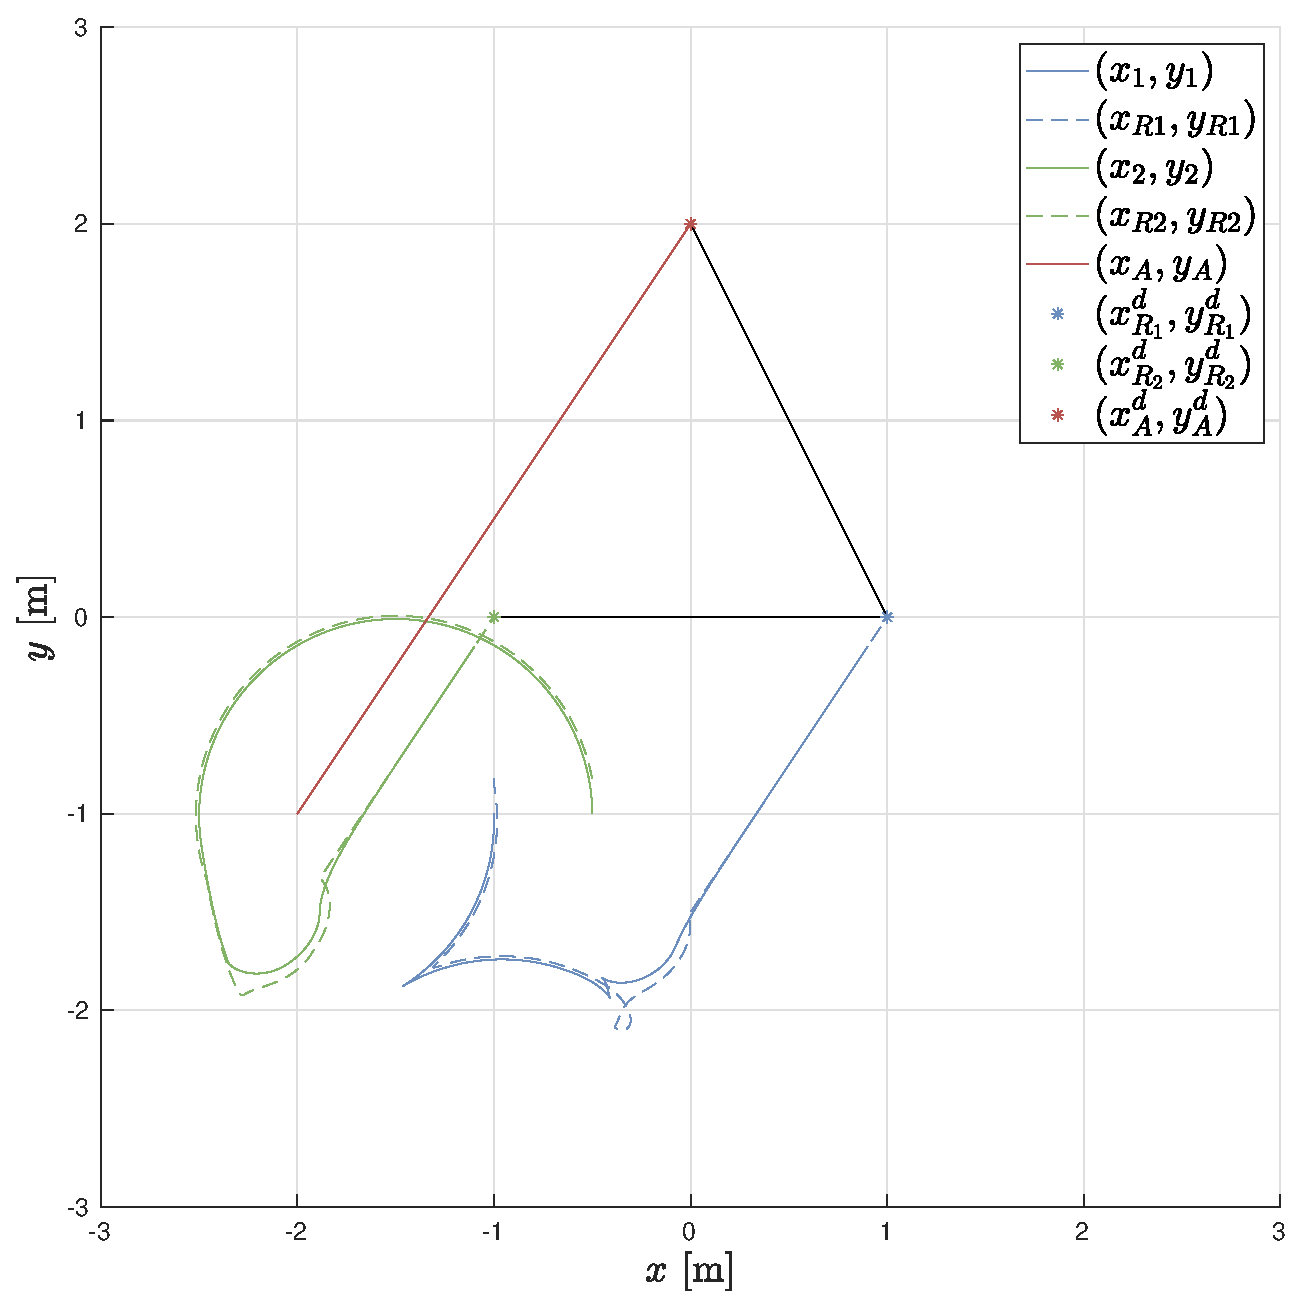
\includegraphics[width=\linewidth]{images/simulations/with_APF/1st_scenario_with.eps}
         \caption{Triangle Top}
    \end{subfigure}
    \begin{subfigure}[b]{0.32\columnwidth}
        \centering
        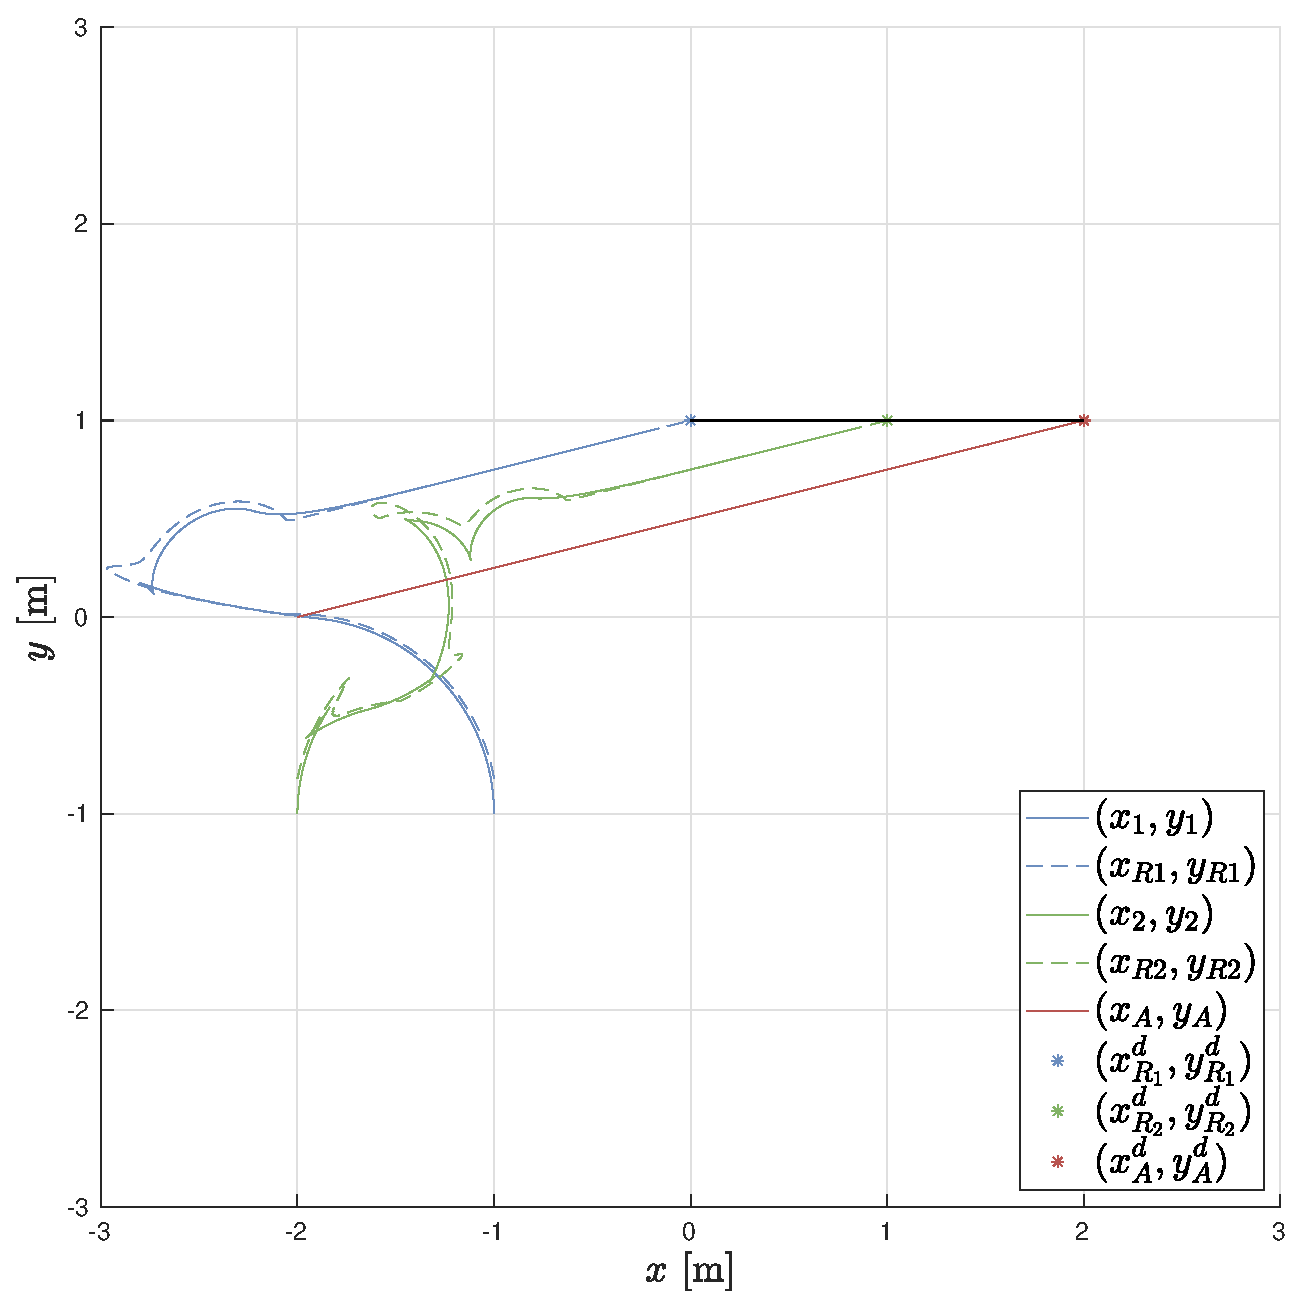
\includegraphics[width=\linewidth]{images/simulations/with_APF/2nd_scenario_with.eps}
        \caption{Line Segment}
    \end{subfigure}
    \begin{subfigure}[b]{0.32\columnwidth}
        \centering
        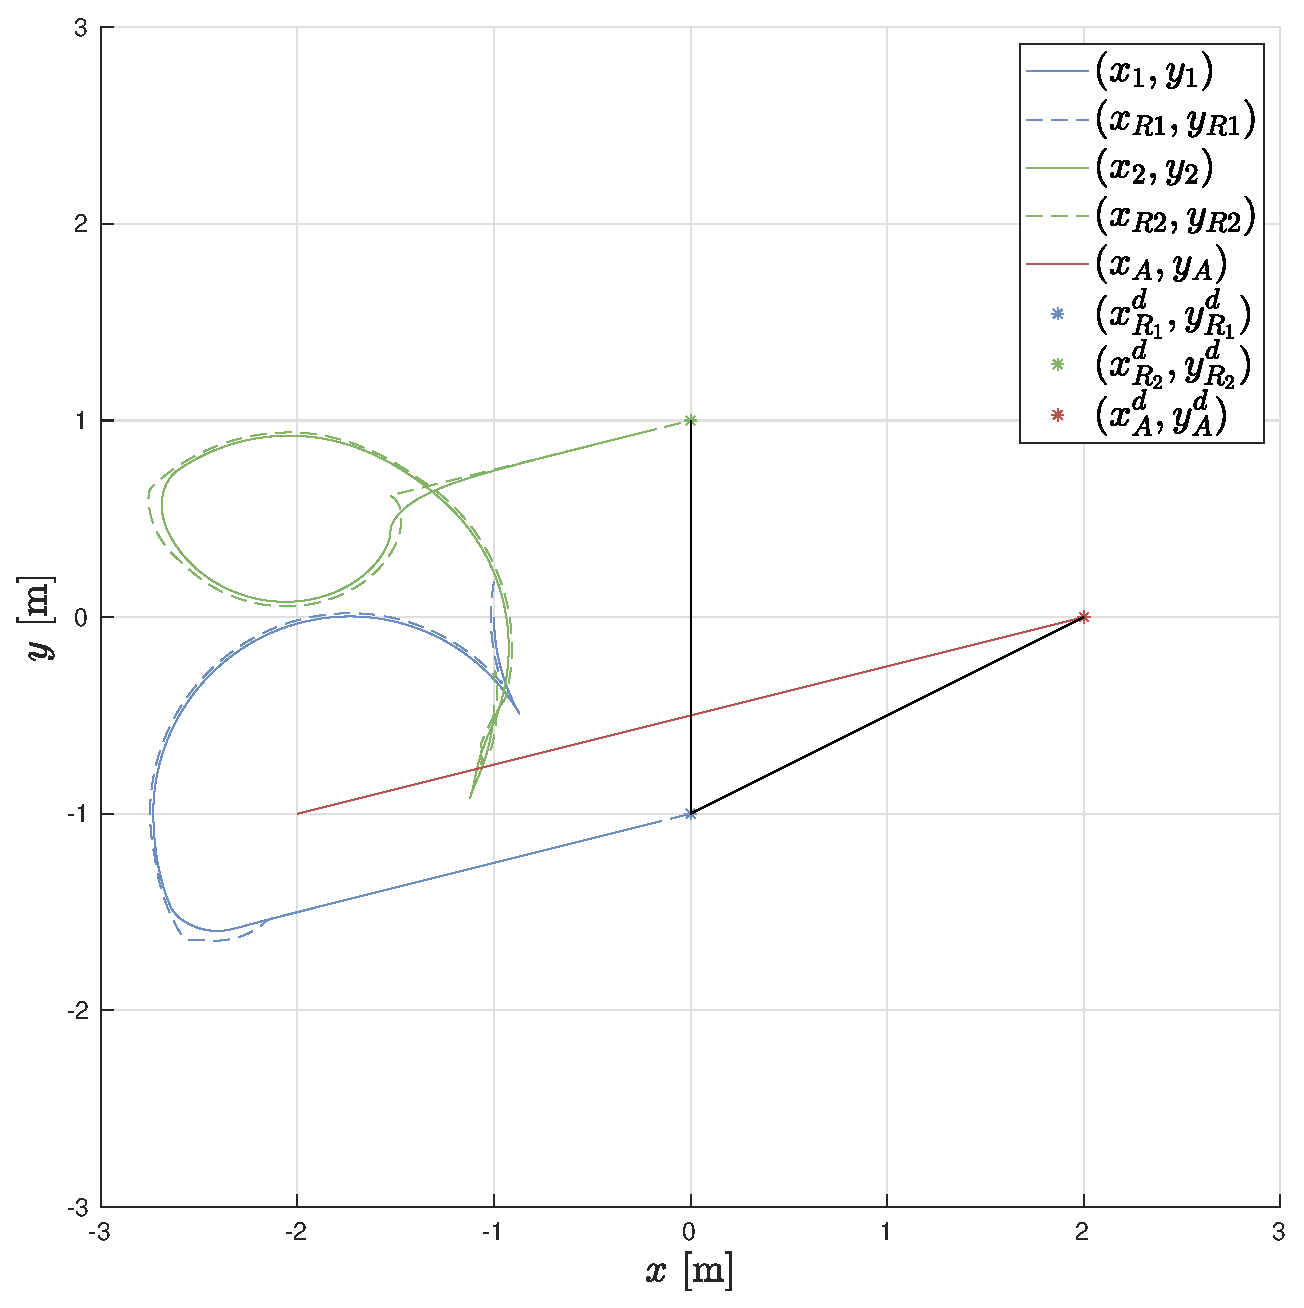
\includegraphics[width=\linewidth]{images/simulations/with_APF/3rd_scenario_with.eps}
      \caption{Triangle Right}
    \end{subfigure}
    \vspace{-0.2cm}
    \caption{Trajectories of the three agents with desired and actual interdistances in simulation.}
\end{figure}

\begin{figure}
    \centering
    \begin{subfigure}[b]{0.32\columnwidth}
        \centering
        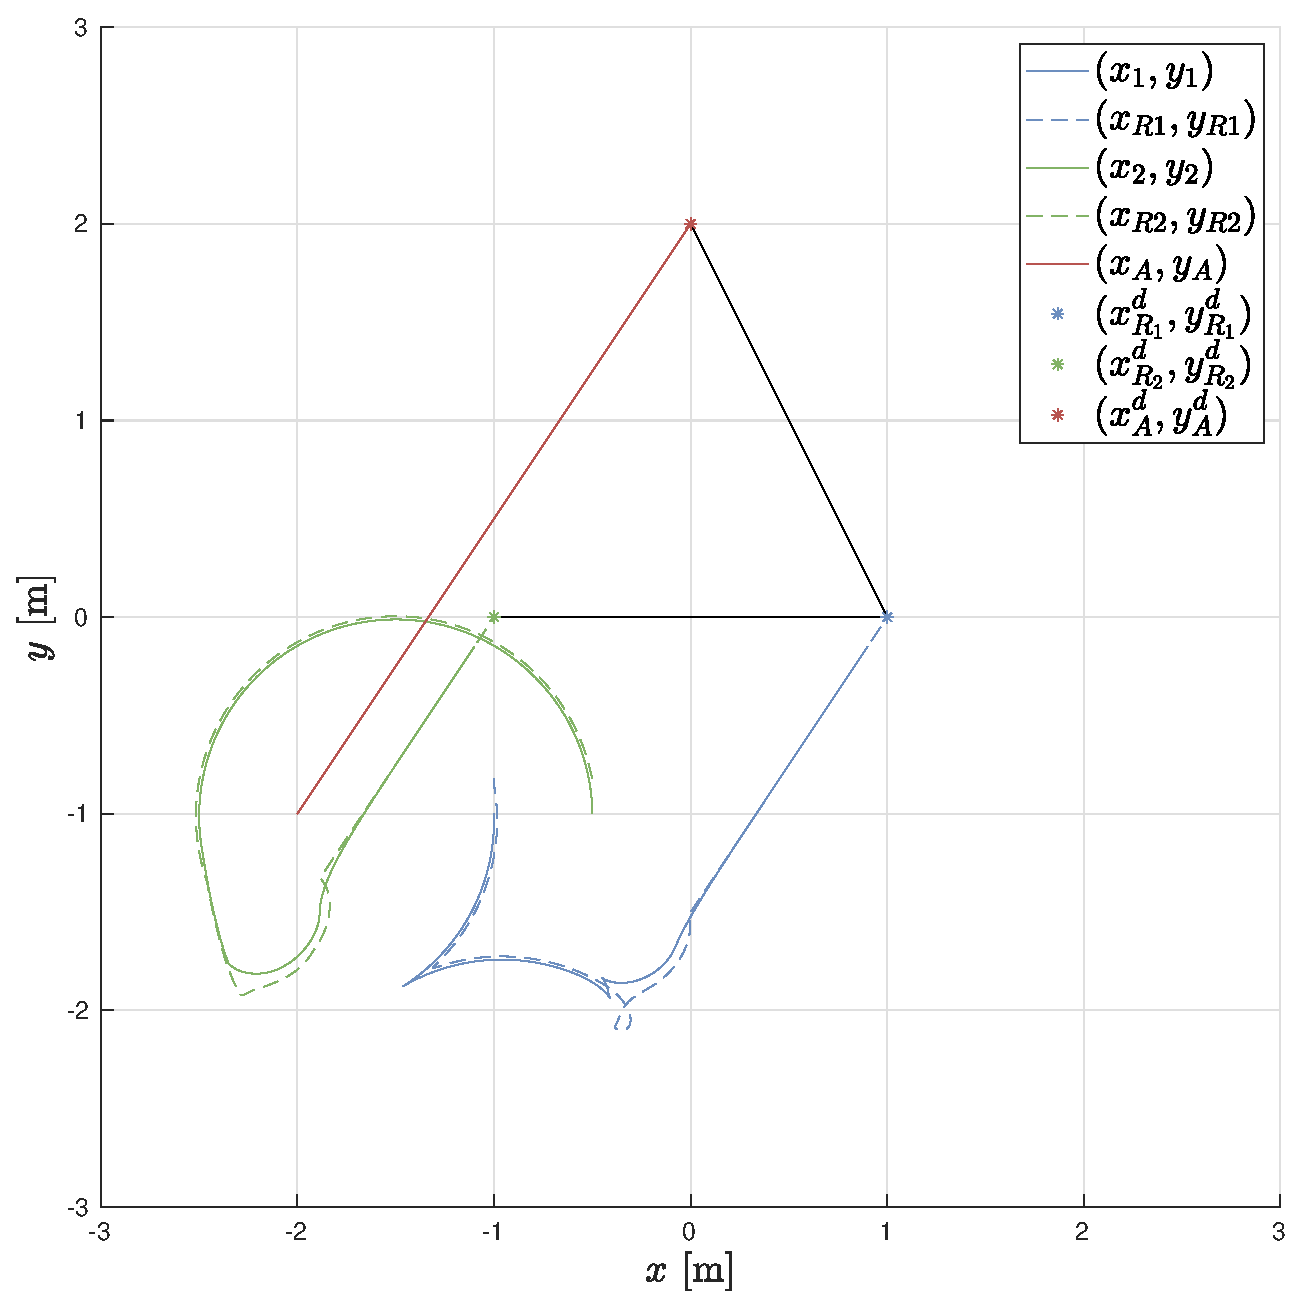
\includegraphics[width=\linewidth]{images/simulations/wo_APF/1st_scenario_wo.eps}
        \caption{Triangle Top}
    \end{subfigure}
    \begin{subfigure}[b]{0.32\columnwidth}
        \centering
        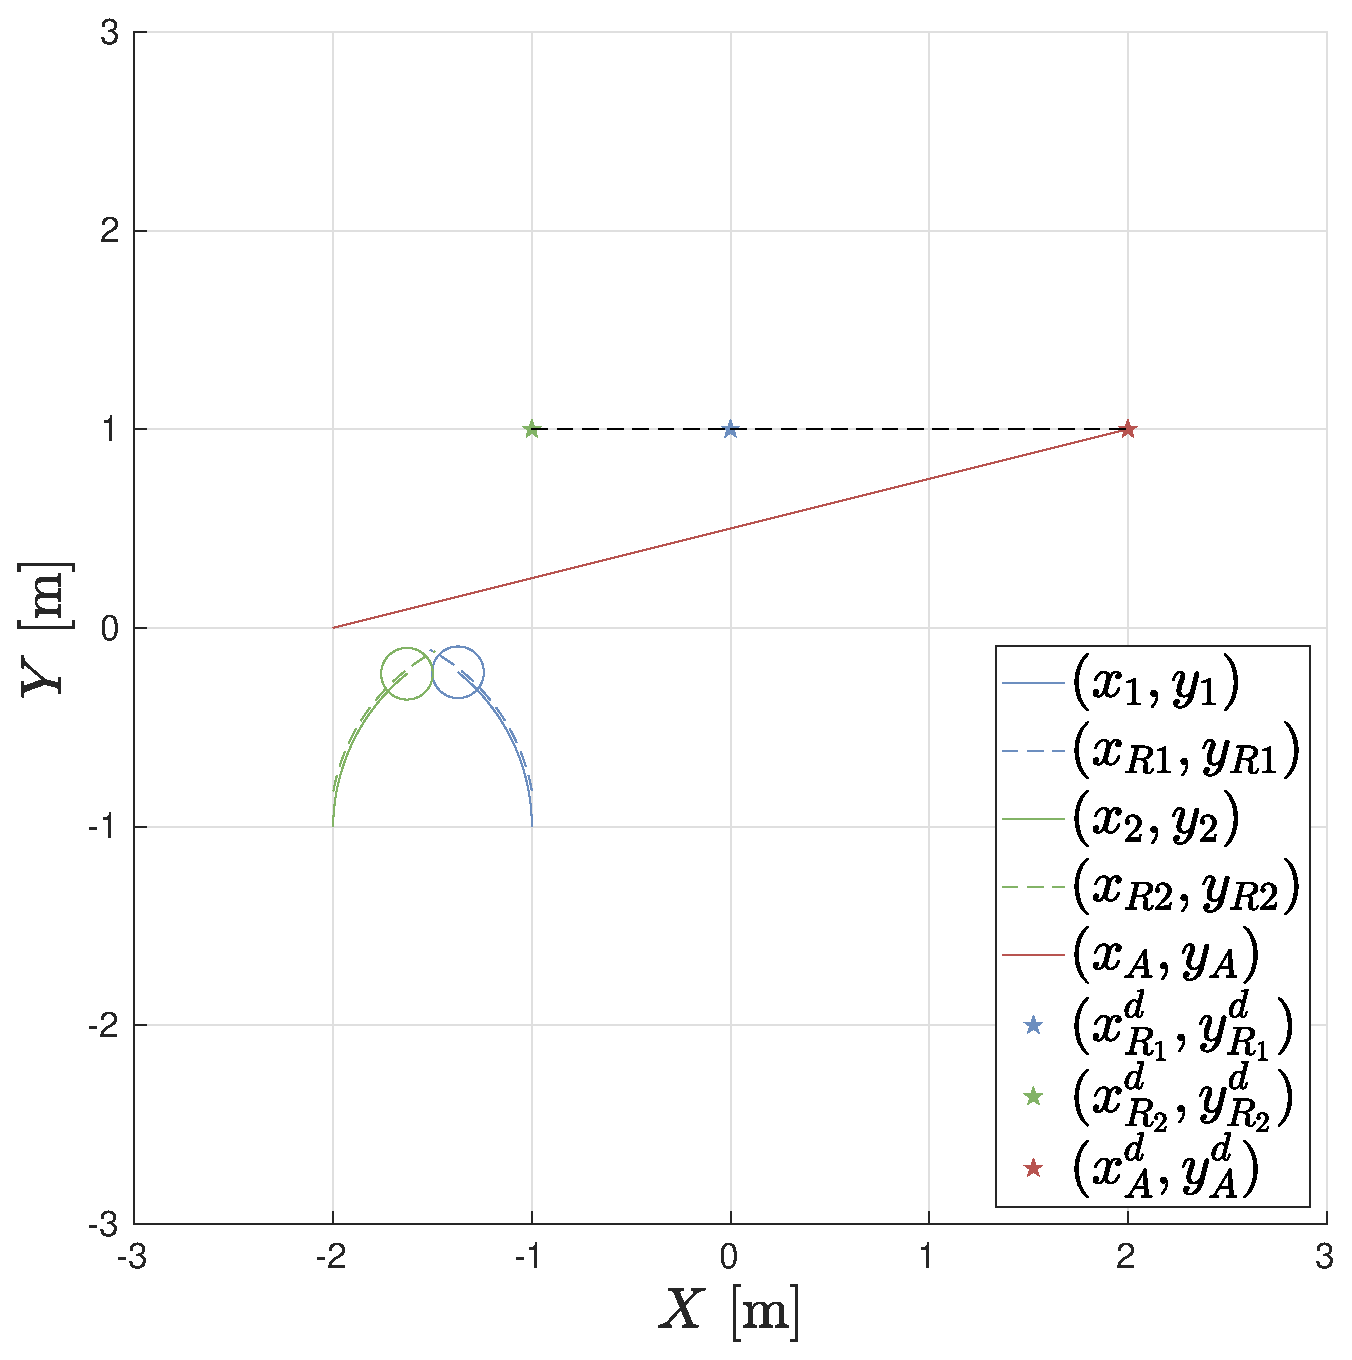
\includegraphics[width=\linewidth]{images/simulations/wo_APF/2nd_scenario_wo.eps}
        \caption{Line Segment}
    \end{subfigure}
    % \hfill
    \begin{subfigure}[b]{0.32\columnwidth}
        \centering
        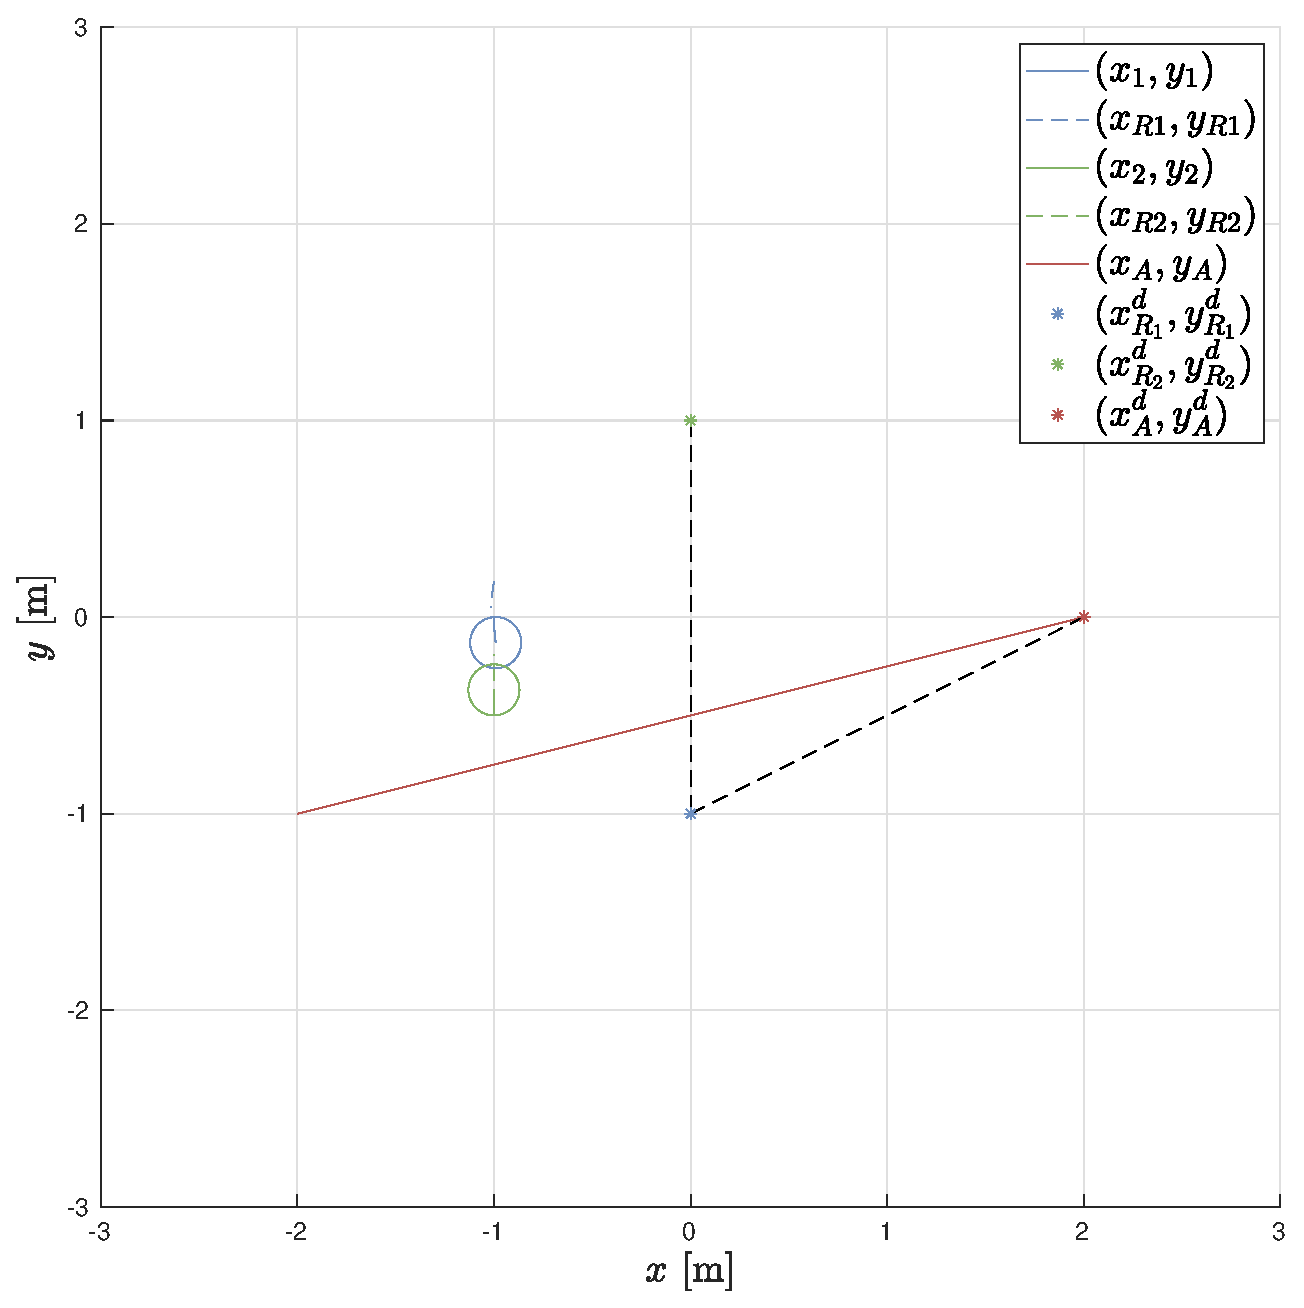
\includegraphics[width=\linewidth]{images/simulations/wo_APF/3rd_scenario_wo.eps}
        \caption{Triangle Right}
    \end{subfigure}
    \vspace{-0.2cm}
    \caption{Trajectories of the three agents without APF in simulation.}
\end{figure}


\section{Experimental Validation}
\label{sec:experimental_validation}
\textcolor{red}{dire che usi FL-AIR per il drone, pensa se incrementare $\varepsilon$ a 20cm invece di 17cm}
\begin{figure}
    \centering
    \begin{subfigure}[b]{0.31\columnwidth}
        \centering
        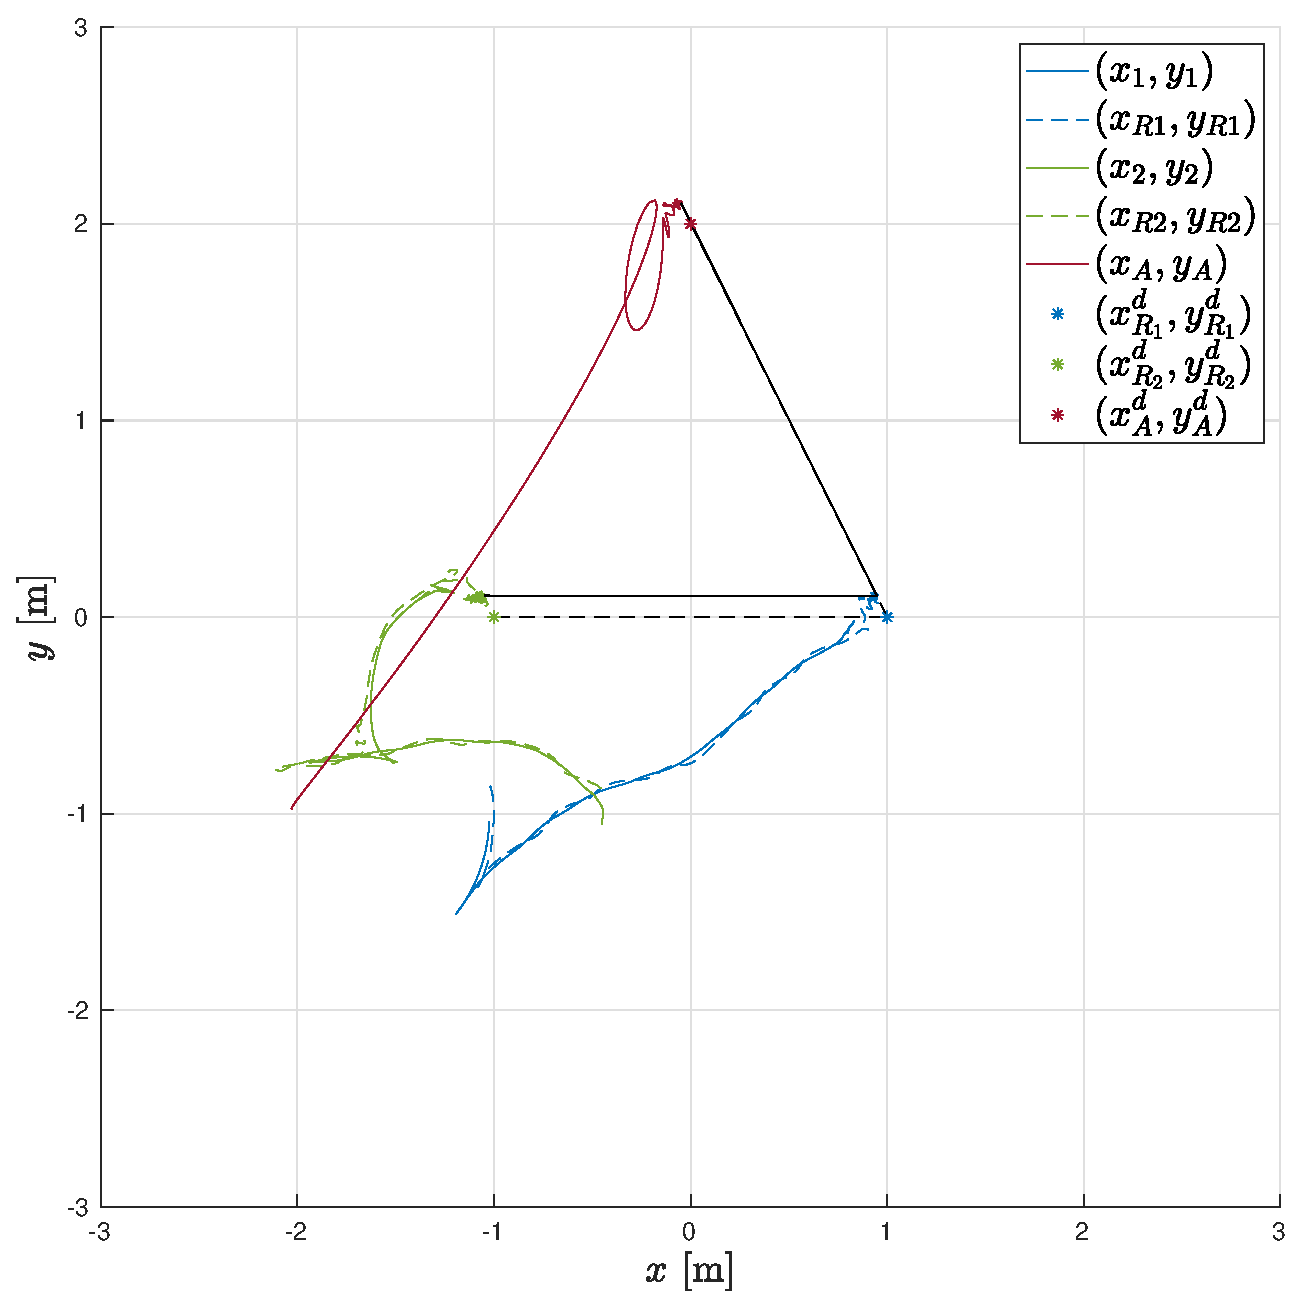
\includegraphics[width=\linewidth]{images/experiment/nominal/1st_scenario_exp.eps}
        \caption{Triangle Top}
    \end{subfigure}
    \begin{subfigure}[b]{0.31\columnwidth}
        \centering
        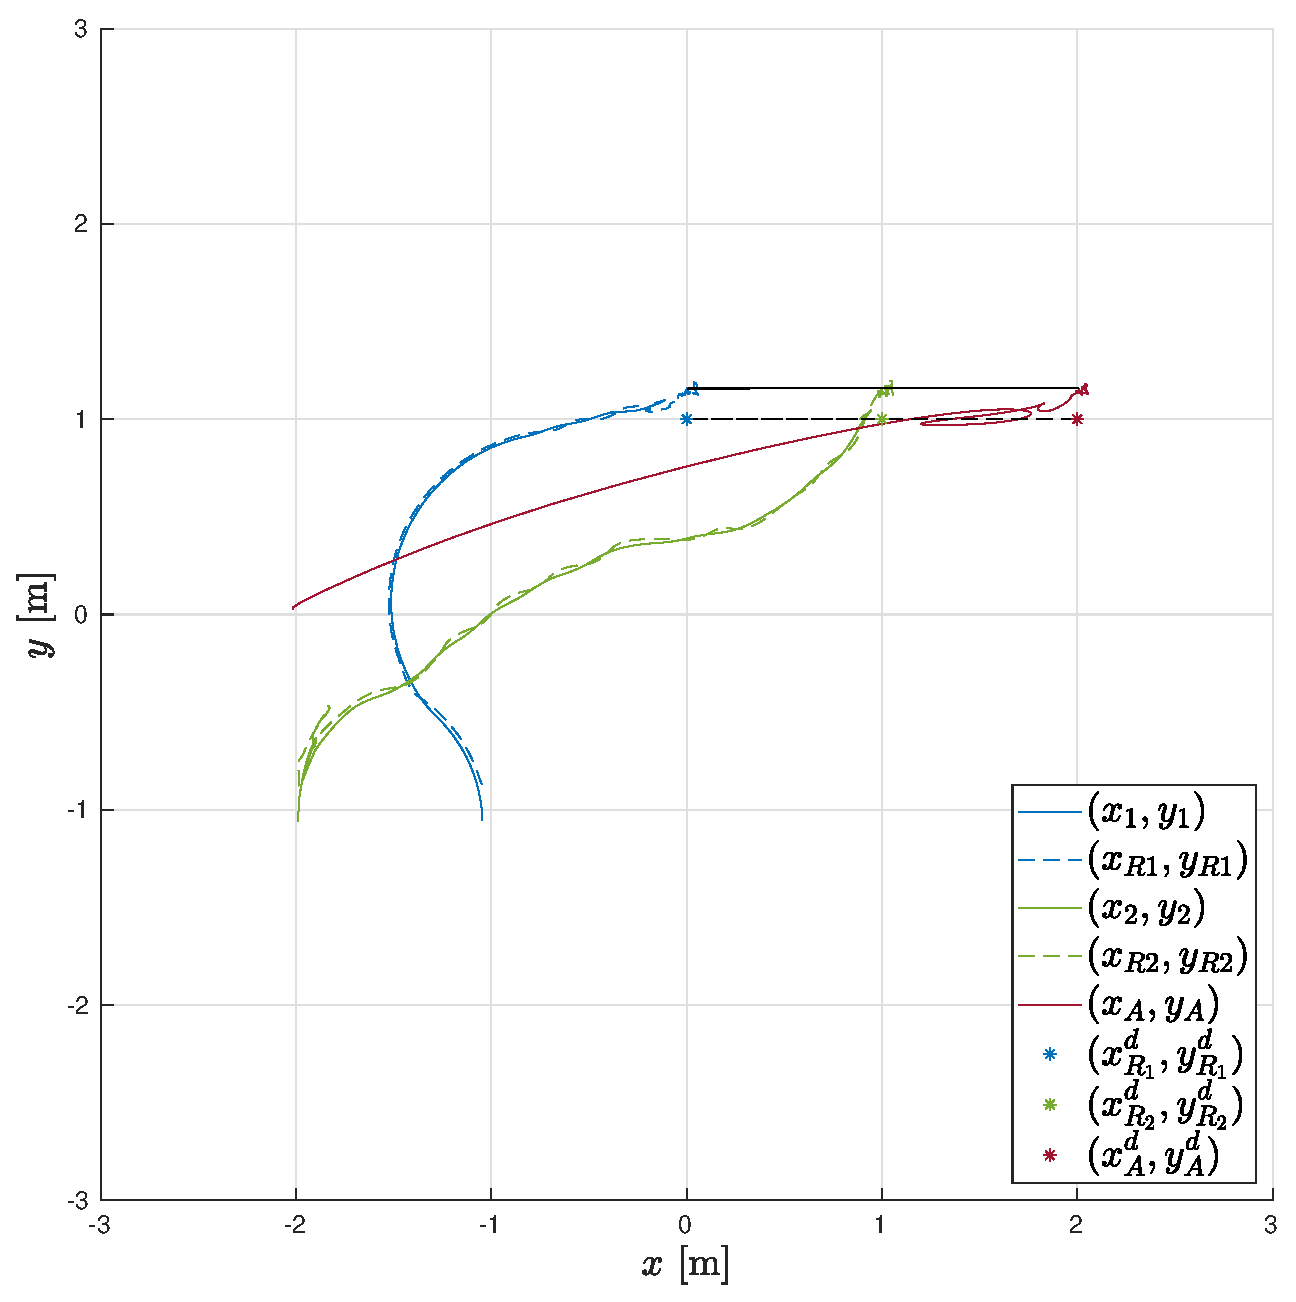
\includegraphics[width=\linewidth]{images/experiment/nominal/2nd_scenario_exp.eps}
      \caption{Line Segment}
   \end{subfigure}
    \begin{subfigure}[b]{0.31\columnwidth}
        \centering
        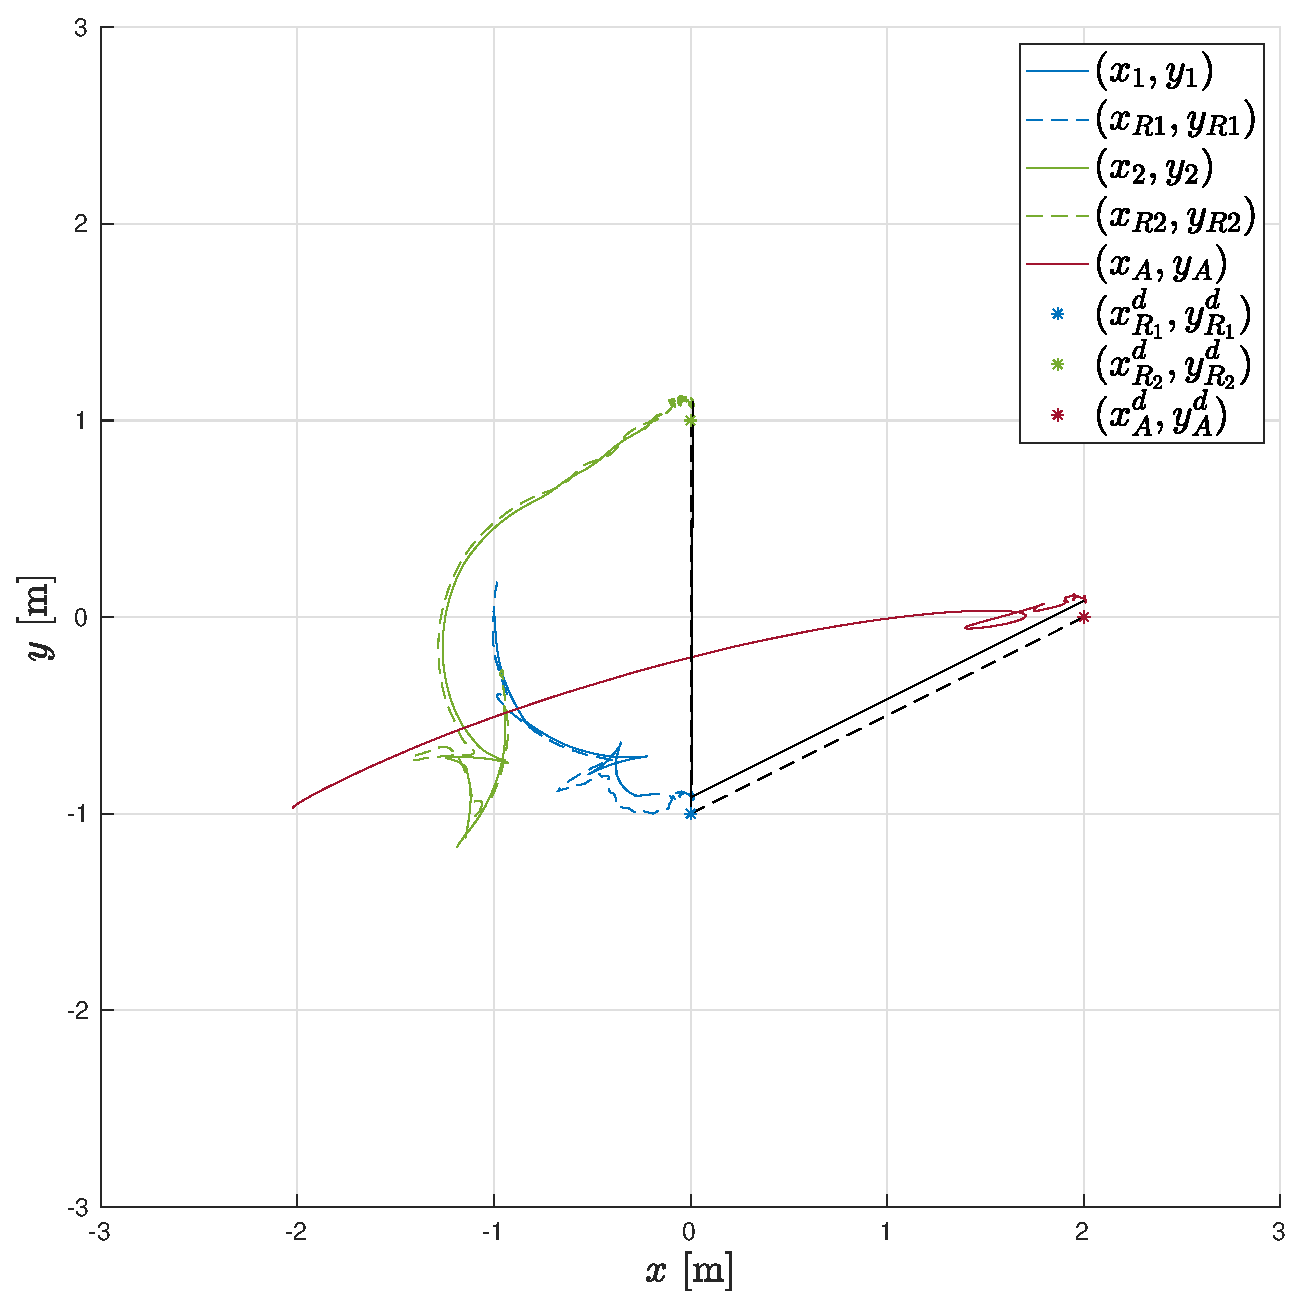
\includegraphics[width=\linewidth]{images/experiment/nominal/3rd_scenario_exp.eps}
        \caption{Triangle Right}
      \end{subfigure}
   \vspace{-0.2cm}
   \caption{Trajectories of the three agents with desired and actual interdistances in the experiments.}
\end{figure}

For each obstacle, just add a corrective APF term: \textcolor{red}{add formula}

Increased $y_A^d$ of $\SI{0.5}{\meter}$, 
formation reached after \SI{55.30}{\second}(the drone 
takes some time, but $R_2$ achieve the formation w.r.t 
$R_1$ after \SI{16.02}{\second}), when swapped
the formation is achieved after \SI{9.74}{\second} 
(drone after \SI{8.32}{\second}
while $R_2$ after \SI{9.74}{\second}).


\begin{figure}[h!]
    \centering
    \begin{subfigure}[b]{0.31\columnwidth}
        \centering
        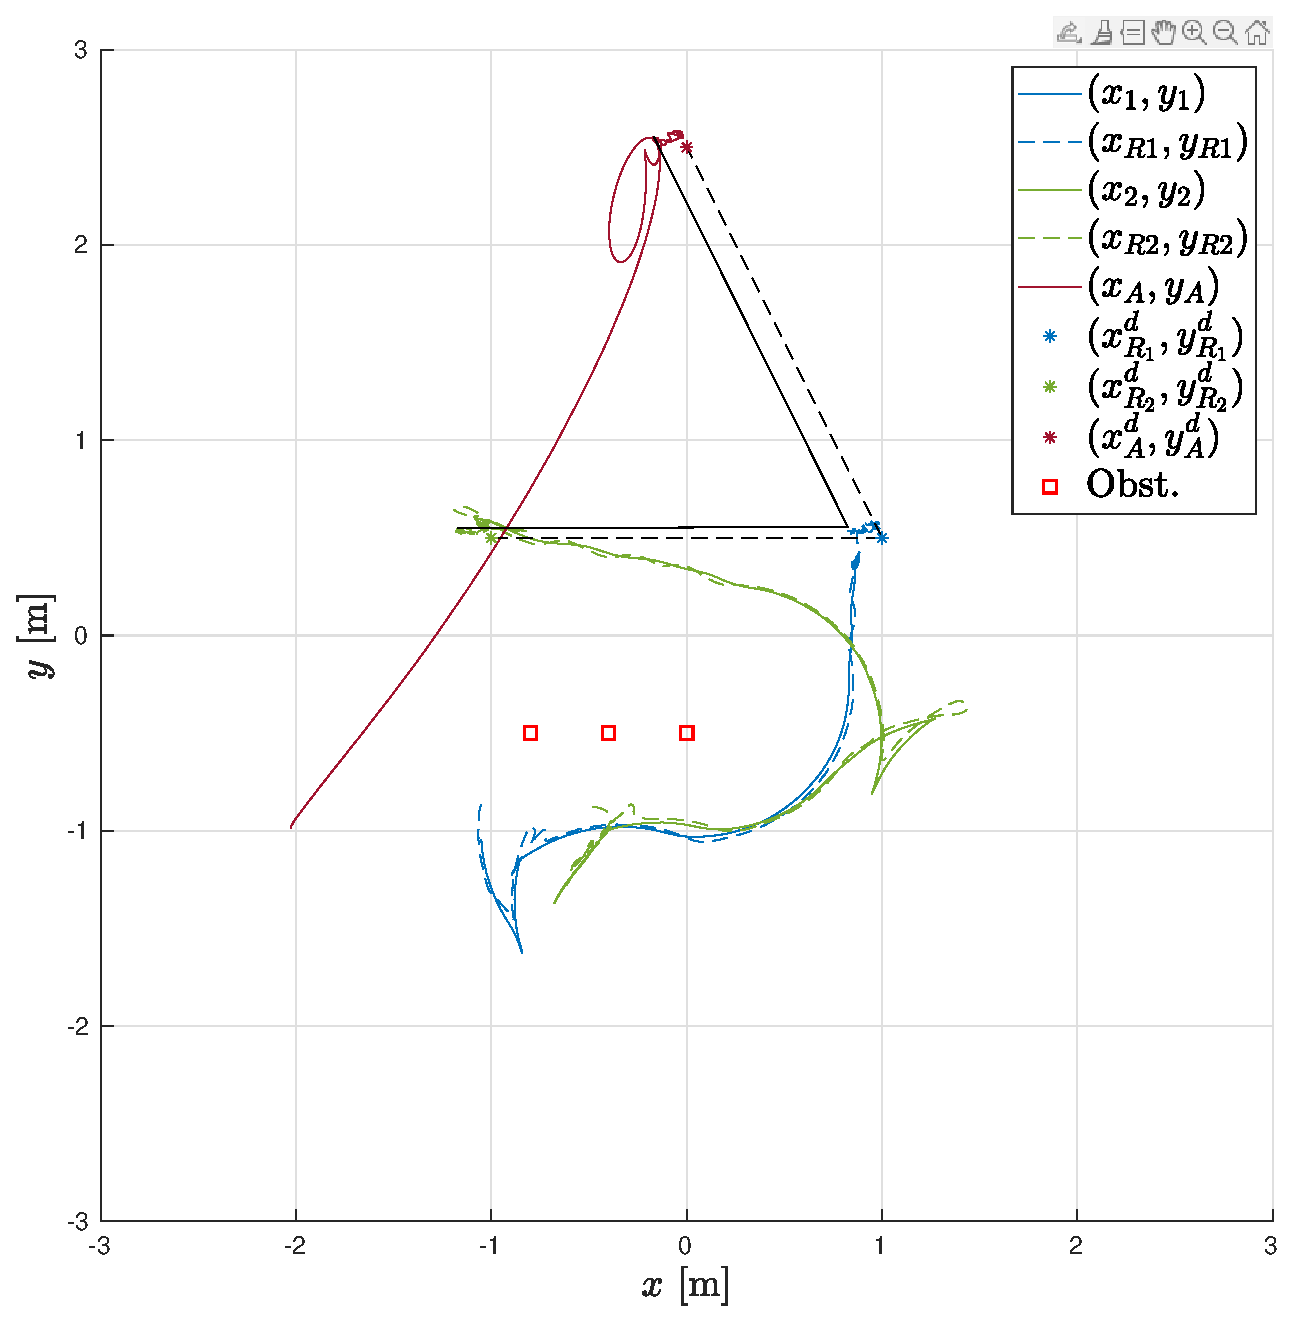
\includegraphics[width=\linewidth]{images/experiment/static_obstacles/1st_scenario_obs_exp.eps}
        \caption{$R_2$ on the right}
    \end{subfigure}
    \begin{subfigure}[b]{0.31\columnwidth}
        \centering
        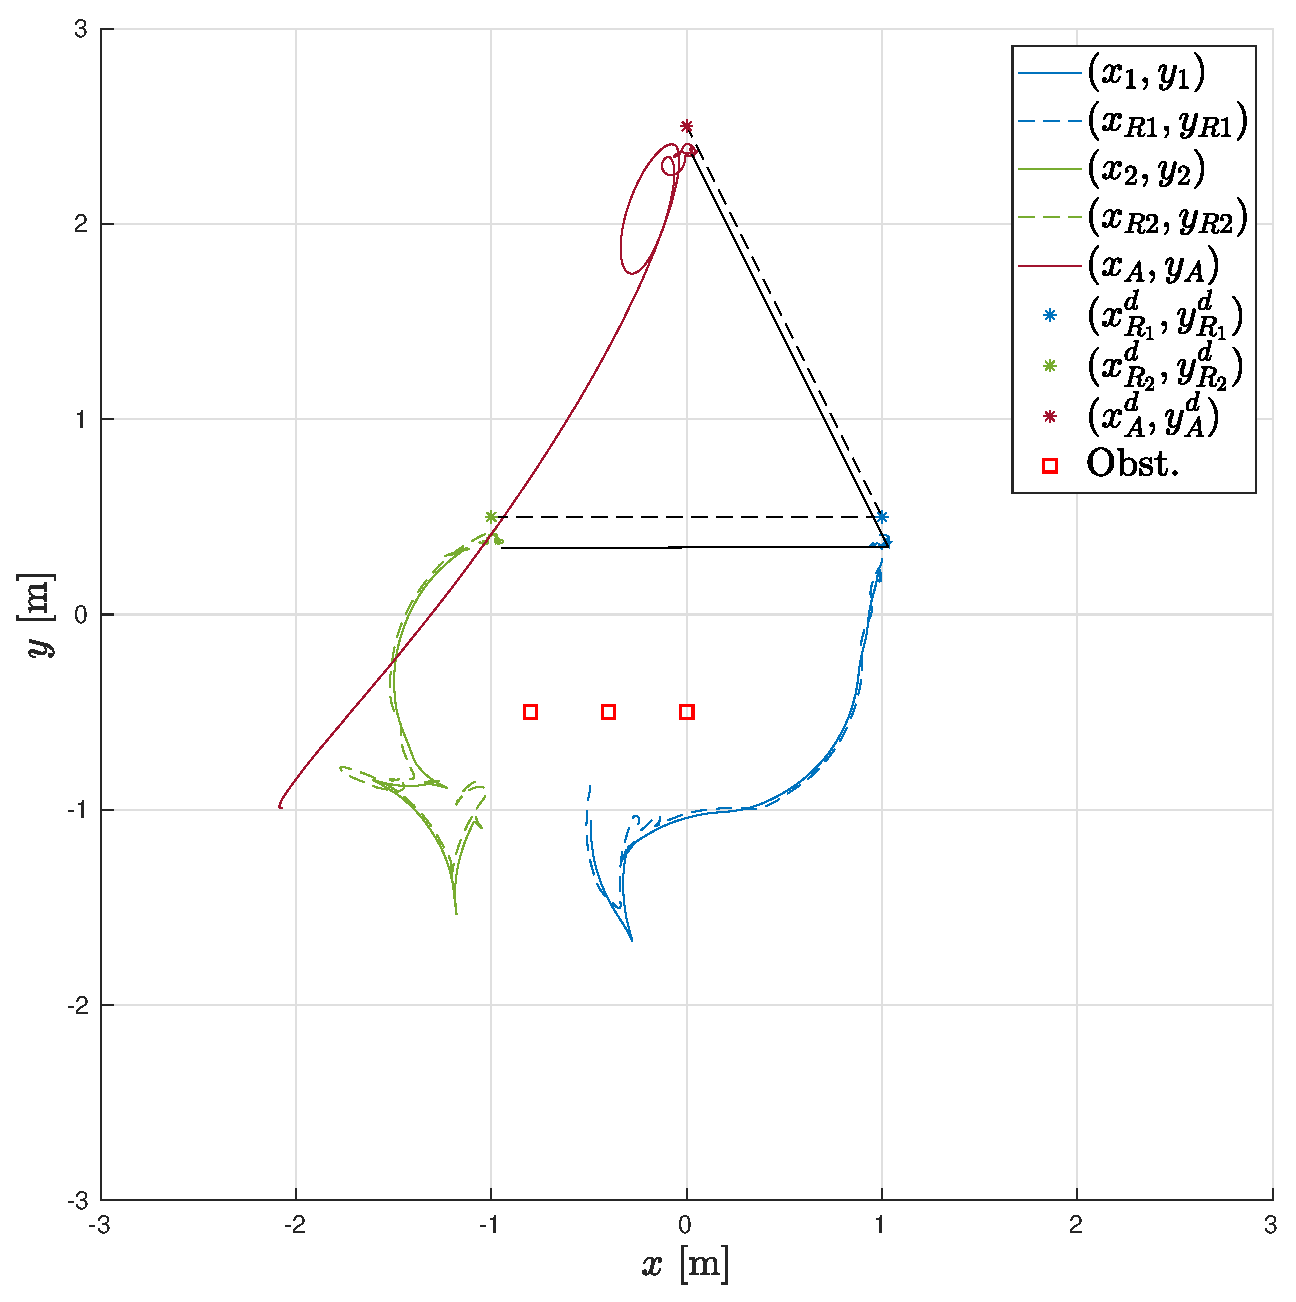
\includegraphics[width=\linewidth]{images/experiment/static_obstacles/1st_scenario_exp_obs_swap.eps}
        \caption{$R_2$ on the left}
    \end{subfigure}
    \vspace{-0.2cm}
    \caption{\textcolor{red}{TODO}}
\end{figure}


\section{Conclusion}
\label{sec:conclusion}

\dots

\bibliography{bibliography}    % bib file to produce the bibliography
                           % with bibtex (preferred)

\end{document}
